% !TeX root = ../main.tex
% Add the above to each chapter to make compiling the PDF easier in some editors.

\chapter{Implementation}\label{chapter:implementation}

This chapter explains different solutions for the problem at hand. These solutions include applications using different datasets and different methods.

As we mentioned in the Introduction part [See~\autoref{section:motivation}], the implementation of this thesis focuses on recommending the best talents to projects. While serving this aim, we use different datasets and different methods. 


The methods used can be categorized as individual and group recommenders. Individual recommenders have the aim of suggesting only one person to a project. As oppose to that, group recommenders combine multiple subprojects as a super project and recommend various talents to this super project. Another differentiation of these recommenders is the type of learning algorithms. Both group recommenders and the individual recommenders are implemented via supervised and unsupervised learning approaches. The supervised learning approach trains neural networks with the help of ground-truth labels. On the other hand, the unsupervised approach employs training just with the feature vectors ~\parencite{sathya2013comparison}. Detailed information about these methods can be found in the upcoming sections. 

\section{Datasets}\label{section:datasets}

The author of the thesis received two separate but similar datasets before starting the thesis. Both of the datasets contain information about projects and people. The company dataset [See~\autoref{subsection:company-dataset}] is the internal database of the company Motius and includes skill vectors of 795 people and 375 roles. These roles come together and form projects, which is not the case in freelancer dataset. In freelancer dataset, we have projects as opposed to positions in the company dataset. However, we treat the projects in the freelancer data and the roles in the company data the same. The reason for that is that we want to combine both data and we also want to compare them.



A huge difference is a fact that the Freelancer dataset is much bigger and detailed compared to the company dataset. The freelancer dataset contains 30606 roles that are comparable to the positions in the company dataset. It has 32922 unique talents and 463536 bids by talents to the projects that represent the project-talent pairs.



Another significant contrast between the two datasets is the distribution of their positive and negative labels. Freelancer data carries approximately 14-15 applicants per projects, and only one of the applicants get selected as the person to implement the project. Differently,  the company dataset includes multiple talents that advance to the next steps of the interviews. Therefore, we marked all of these talents that got invited with a positive label, and we marked the rest with negative tags. We will give detailed information about both datasets in the upcoming subsections.


\subsection{Freelancer Dataset}\label{implementation-subsection-freelancer}


\begin{figure}[!ht]
	\centering
	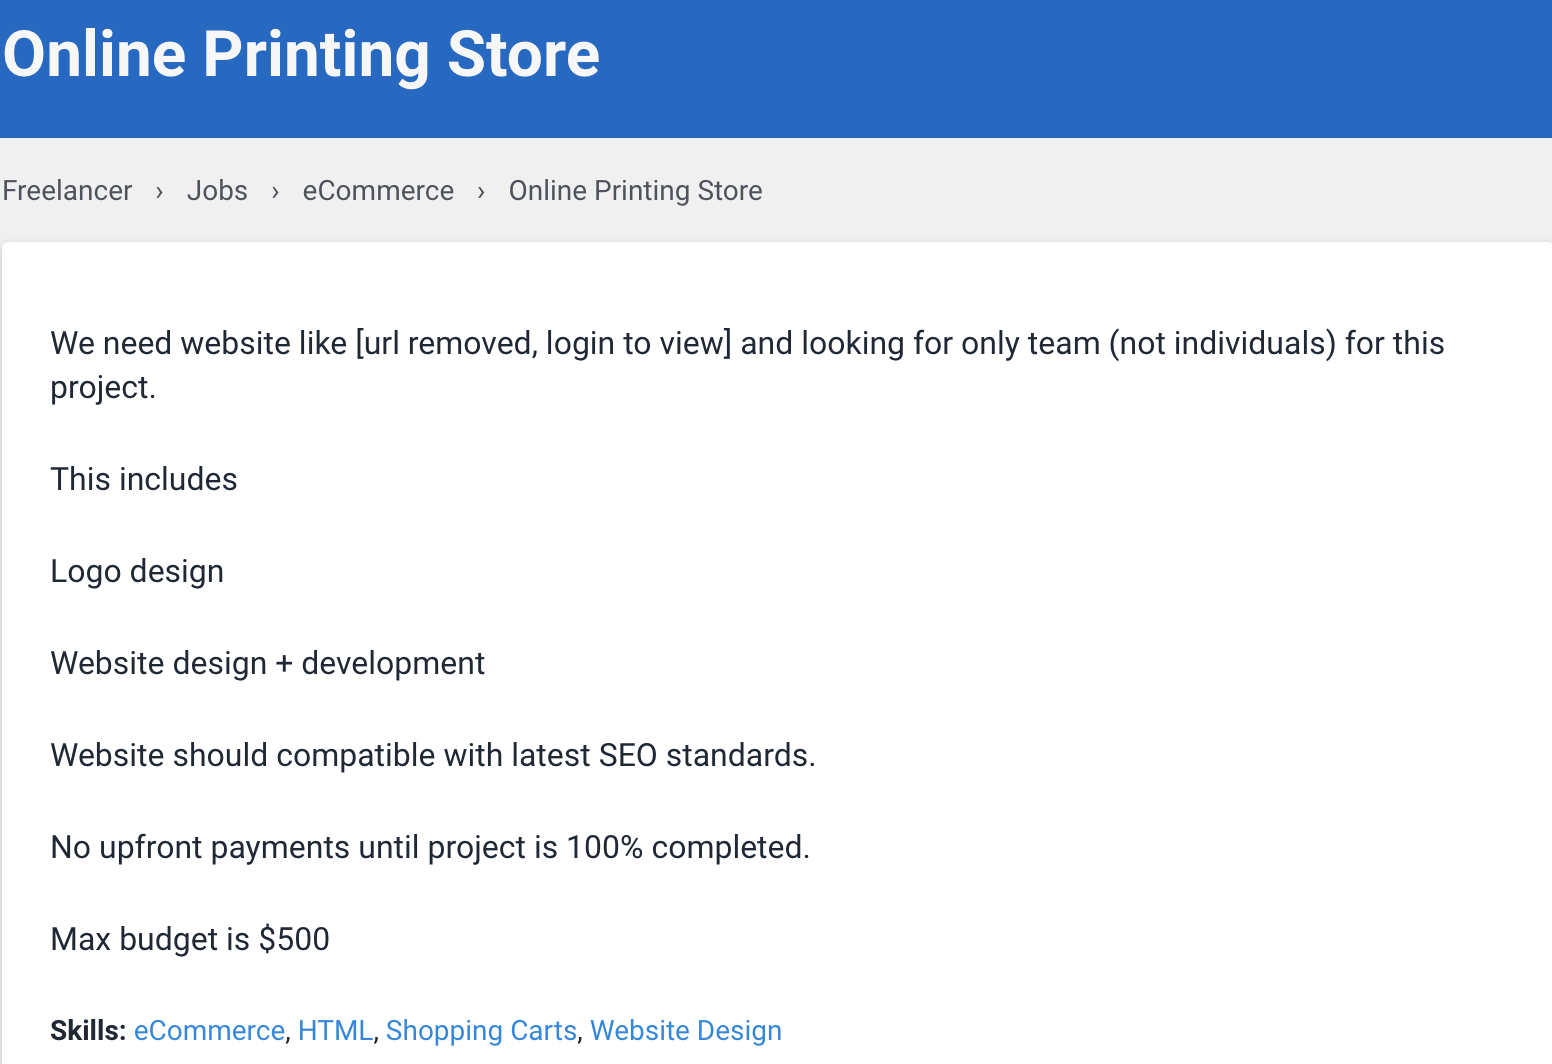
\includegraphics[width=\textwidth]{figures/FreelancerExample.png}
	\caption{An example project from the Freelancer Website}
	\label{fig:freelancer-example-project}
\end{figure}


As you can see in the figure \ref{fig:freelancer-example-project}, a typical freelancer project posting consists of a title, the description and the relevant skills. For simplicity, the thesis at hand only concentrates on the skills and doesn't take the project description into account. This would be topic of another paper/thesis, as it would require natural language processing and other techniques ~\parencite{bird2009natural}.


\begin{figure}[!ht]
	\centering
	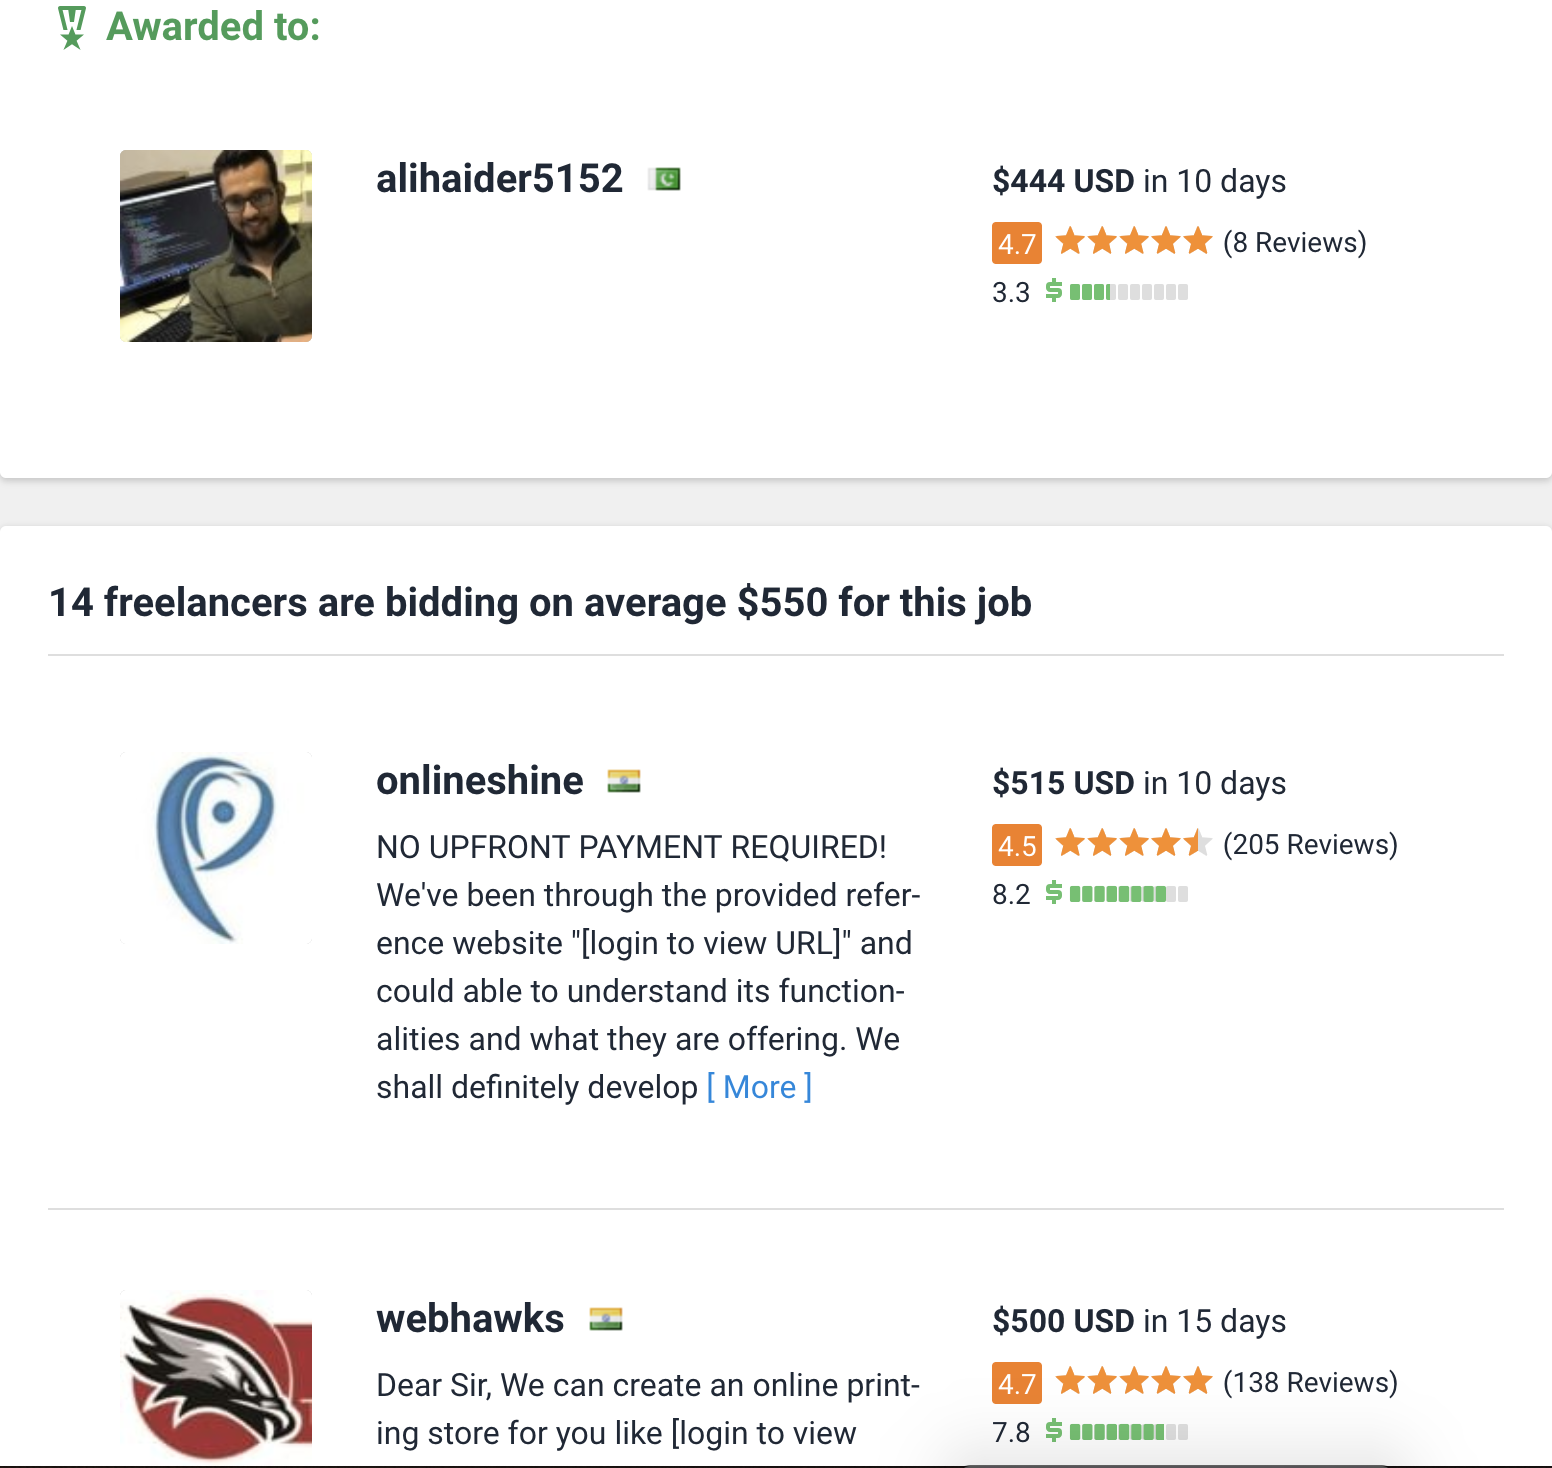
\includegraphics[width=0.75\textwidth]{figures/FreelancerTalentExample.png}
	\caption{The winner and other bidders to the same project}
	\label{fig:freelancer-example-talent}
\end{figure}


The figure \ref{fig:freelancer-example-talent} shows the bidders of the same project as above. The first one of the bidders has won the bidding race, which is decided by the creator of the project. The bidders include information such as a motivation text, the demanded monetary amount, their star rating until the time of bidding, amount of reviews they received and their total earnings until that date. In this thesis, we only consider the money they demand, their star rating and the number of reviews. For the sake of simplicity, we don't use the motivation text.



Each bidder lists their skills on their profile page, and the employers may check their profiles before hiring talents. The figure depicts the top skills of an arbitrary talent, which are listed in descending order. The number near each skill shows how many related projects the talent completed. That's why the amounts can range from one to more than hundreds. 



\begin{figure}[!ht]
	\centering
	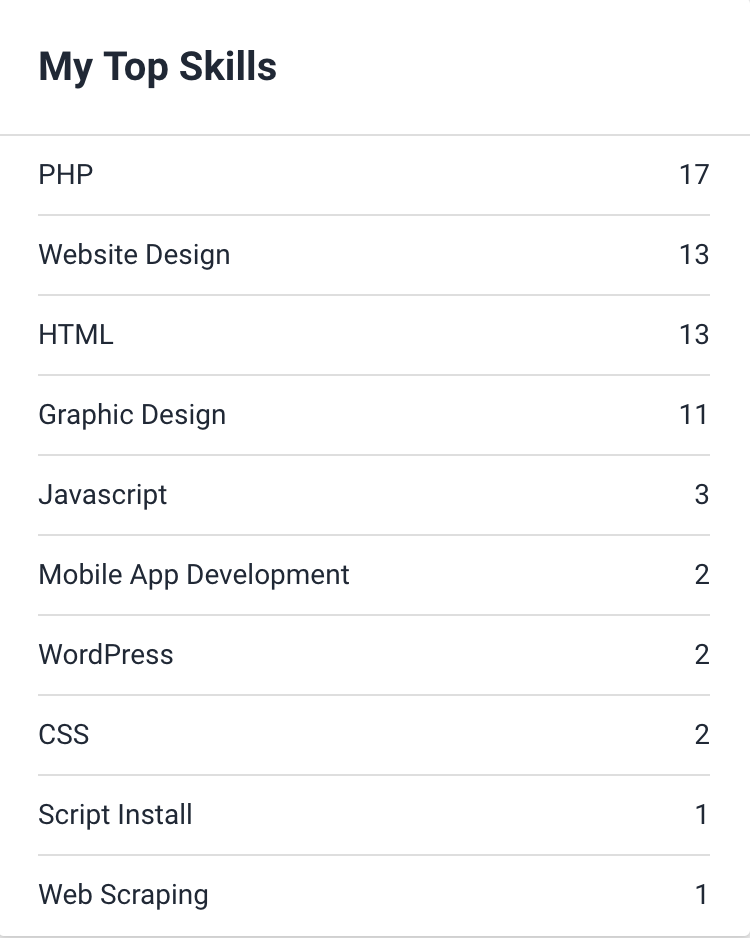
\includegraphics[width=0.5\textwidth]{figures/FreelancerTalentSkills.png}
	\caption{The list of tops skills by a talent on Freelancer web page}
	\label{fig:freelancer-talent-talent}
\end{figure}


The dataset encloses  941 unique skills, which are both technical and non-technical. However, the author of the thesis chose to limit these skills to 780, since some of them weren't used in notable amounts and the data can be expressed without using those skills. [TODO see dimensionality reduction add to research]


This dataset was scraped from freelancer.com by Philip Offtermatt, who also took part in this very project.


\subsection{Company Dataset}\label{subsection:company-dataset}

The company dataset at hand is acquired from the sponsor of this thesis, which is Motius GmbH. This dataset exported from their internal database and contains information of 795 people and 375 roles. Each role includes the required skills for them, and each person has their skills listed. One difference to the freelancer dataset would be that the talents also include skills that are associated with their original skill set. In theory, this is called association rules, and the skills that are mostly used together are considered to have a correlation score of 1. Because of these correlations, each talent has many skills listed, some of them highly correlated and others are not correlated at all.


The amount of unique skills in the company data equals to 1768. Nonetheless, more than 85\% of the skills are used rarely, so the author reduced the unique set of skills to  202. Both of the datasets combined, 923 unique skills were given at least five times. A problem we have with the datasets is the naming. Since both Freelancer and Motius have used different names for skills, there are exists only a set of 59 common skills. Therefore, training both datasets together doesn't improve model like it's expected[TODO: evaluation neural network 10 000 data training, etc.].



When all of freelancer and company dataset are put together in their raw form, the matrix that contains all talent and project data reaches the size of 8 GB. Such a significant memory usage created a big problem for the author of the thesis. Since we only had available physical memory of 16 GB, working with an 8 GB matrix wasn't possible. When an operation like normalization is being done, the library \textit{Pandas} applies many copying operations, which doubles the memory usage and crashes. That's why the author employed embeddings as a dimensionality reduction mechanism[See \ref{subsection:using-embeddings}].




\section{Unsupervised Individual Recommender}\label{implementation-unsupervised-individual}

\subsection{Recommendation by Similarity}\label{implementation-unsupervised-similarity}

As it was mentioned before, the unsupervised learning techniques focus on learning without the use of labels. Therefore, in the context of this thesis, we find similarities between projects and talents by using their feature vectors. 



\begin{equation}
\cos (x, y)=\frac{(x \bullet y)}{\|x\|\|y\|}
\end{equation}


The similarity measure we use for this part of the thesis is the cosine similarity ~\parencite{amatriain2011data}. The formula for the cosine similarity is shown above. The inputs  \textit{x and y} in the equation can correspond to a project-talent or a talent-talent pair. The types of input data are document vectors of an n-dimensional space, and the formula calculates the similarity as the cosine of the angle between two vectors. The recipe first calculates the dot product of the vectors and then divides it by the multiplication of the normal vectors.


To get the most important talents for the project, we calculate the cosine similarity between a selected project and every other talent. Then the algorithm sorts the people by similarity and returns \textit{top n} bidders.



\subsection{Recommendation by Popularity}


Another unsupervised recommendation mechanism that is used as a baseline is the popularity recommender. The popularity recommender is hard to beat algorithm, that increases user satisfaction. [TODO add pages 394 and 395 to research section(from book)]]. The logic comes from the fact that the \textit{items} that are in demand approved by many \textit{people}. That's why it's likely that selecting these items will increase user satisfaction ~\parencite{amatriain2015recommender}. 


For this specific project, the popular items that are in demand are the people that finished the maximum amount of projects at Freelancer or Motius. Although the results won't be personal, recommending the same successful talents is a helpful strategy to acquire proven talents. The proof of this approach is shown in subsection \ref{subsubsection:eval-popularity}.


\subsection{Hybrid Recommendation}\label{section:hybrid}

As a last submethod of unsupervised individual recommenders, we can name the hybrid recommender. Hybrid methods are also called as \textit{ensemble learning} methods. This technique combines the results from multiple processes and outputs a new result ~\parencite{beliakov2015aggregation}. For our use case, the author implemented different versions that combine the similarity recommender and the popularity recommender. We can merge both of the recommenders by adding or multiplying the results. It is also possible to give different weights to these sources.


\section{Supervised Individual Recommender}\label{section:supervised}

Supervised learning means creating a model that learns with the help of labels. In our project, the author conceptualized labels as 0 or 1. 1 is for the case of the person got accepted for the project at freelancer.com or Motius. 0 is for the case that the person got rejected. The models try to predict if the talent should be hired for the project or not(1 or 0).


For this task, we use two different versions; one version that takes all the skills as-is, the other one creates embeddings[TODO: embeddings in research chapter]. Both of the methods employ neural networks[TODO: neural networks in the research chapter].


\subsection{Using Sparse Input}

\begin{figure}[!ht]
	\centering
	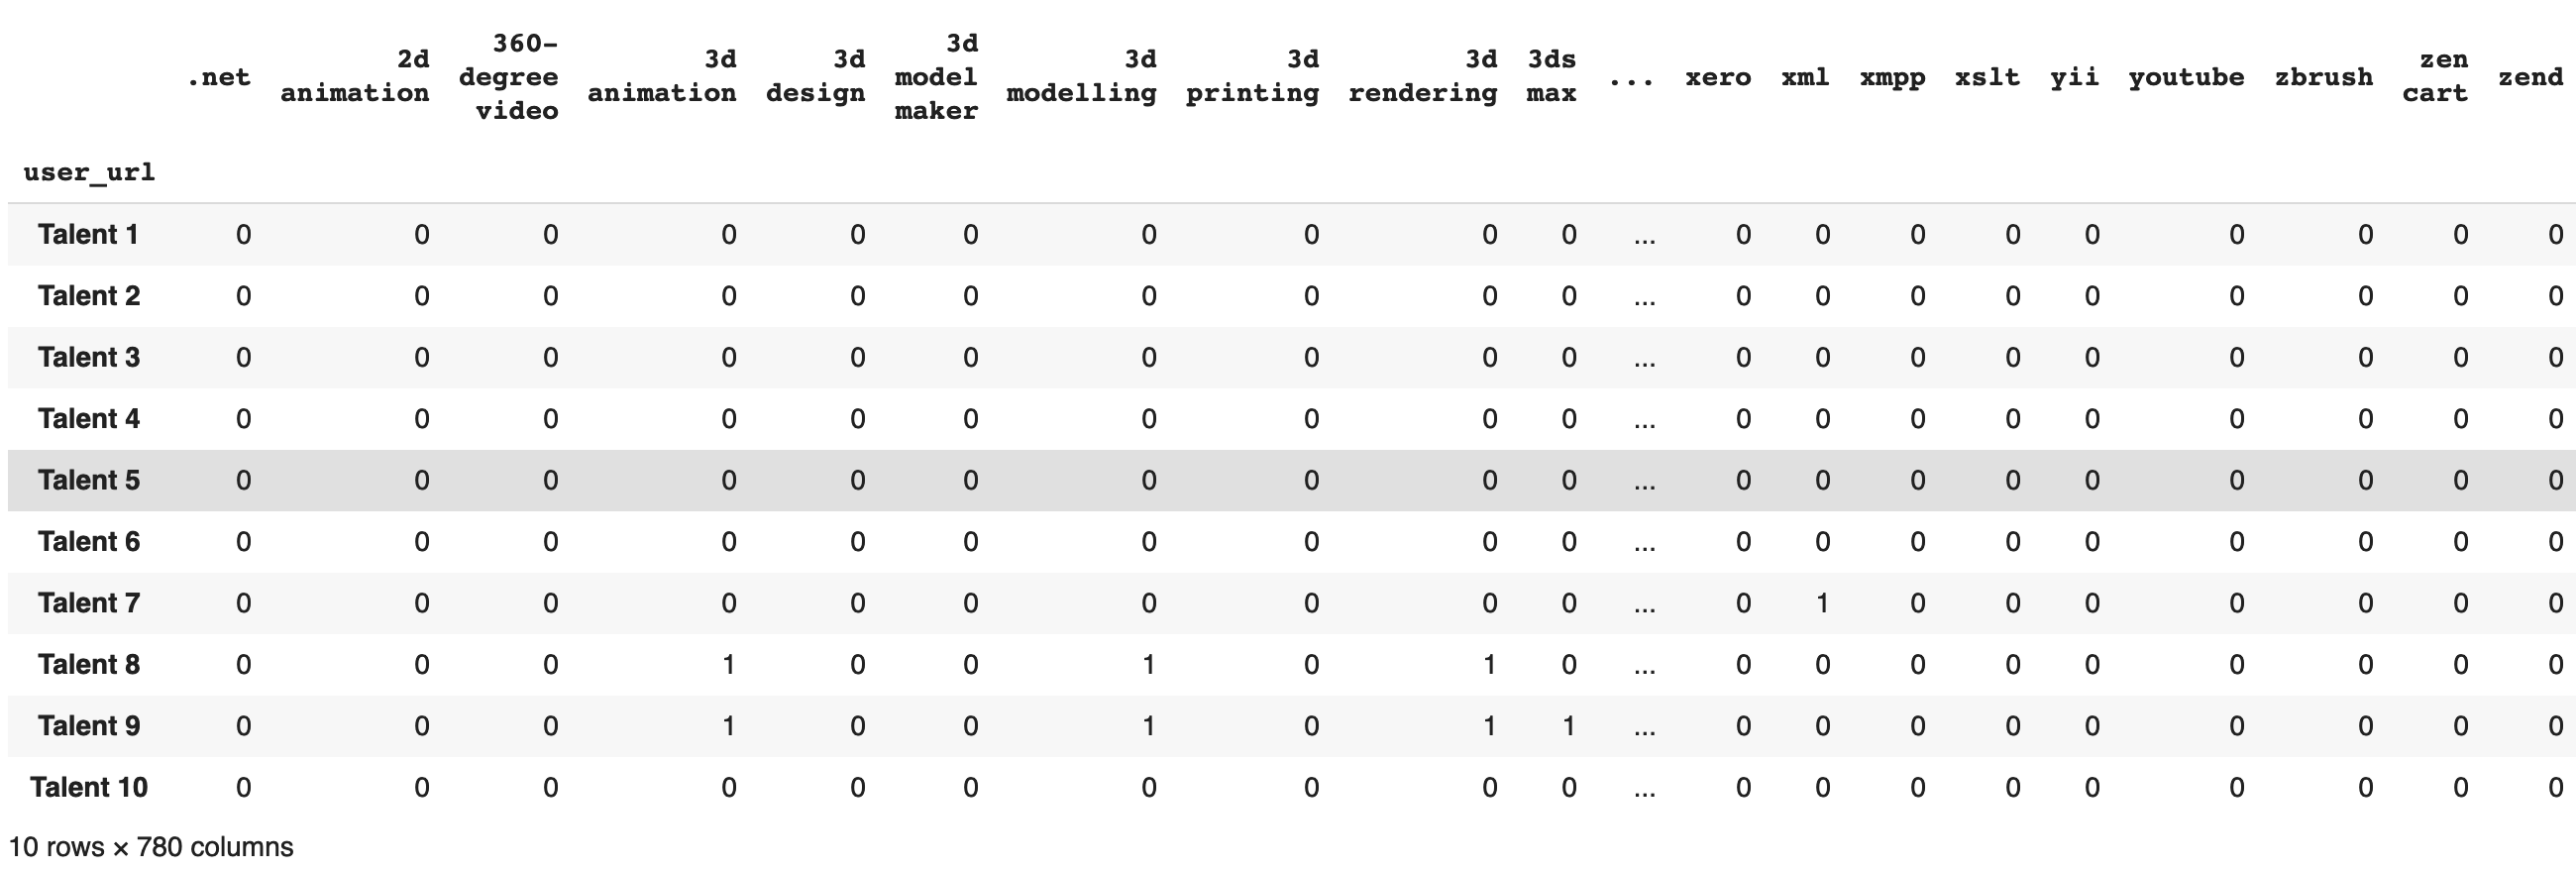
\includegraphics[width=\textwidth]{figures/FreelancerTalentSkillsMatrix.png}
	\caption{The talent skill matrix from freelancer.com}
	\label{fig:freelancer-talent-matrix}
\end{figure}

The first option that comes to mind is using the data as it is and training the model with them. The format of the talent data is shown in figure \ref{fig:freelancer-talent-matrix} and the projects skills matrix also have the same form with project names as keys.


\begin{equation}
z = (x - u) / s
\label{eq:normal}
\end{equation}

According to experts ~\parencite{sola1997importance}, it is crucial to normalize input data before training neural networks. It has two significant benefits; it reduces the estimation errors, and it cuts down the training time. That's why we normalize all of the inputs using \textit{StandardScaler} module of \textit{scikit-learn}. It uses equation \ref{eq:normal} to scale the data. In the equation, \textit{u} is the mean and \textit{s} is the standard deviation.


As it was mentioned before [See section \ref{section:datasets}], the freelancer.com dataset accommodates some extra information like experience level, star rating, number of reviews and hourly rate. These extra information of 10 example talents are shown in the figure \ref{fig:freelancer-talent-meta}. Since this information doesn't exist in Motius dataset, this subsection focuses only on the implementation with freelancer datafset. The extra information that is mentioned is also scaled and input into the neural network. 


After normalizing data, we prepare the matrix that is fed into the neural network row by row. For each bid in the freelancer data, we create a vector of length 1565. Seven hundred eighty of these values correspond to talent skills, the next 780 correspond to project skills, 4 of them are the extra information that is mentioned above and the last of them is for the outcome. The outcome is 1 for the case that the person received the project and 0 for the example that the person didn't receive the project.



\begin{figure}[!ht]
	\centering
	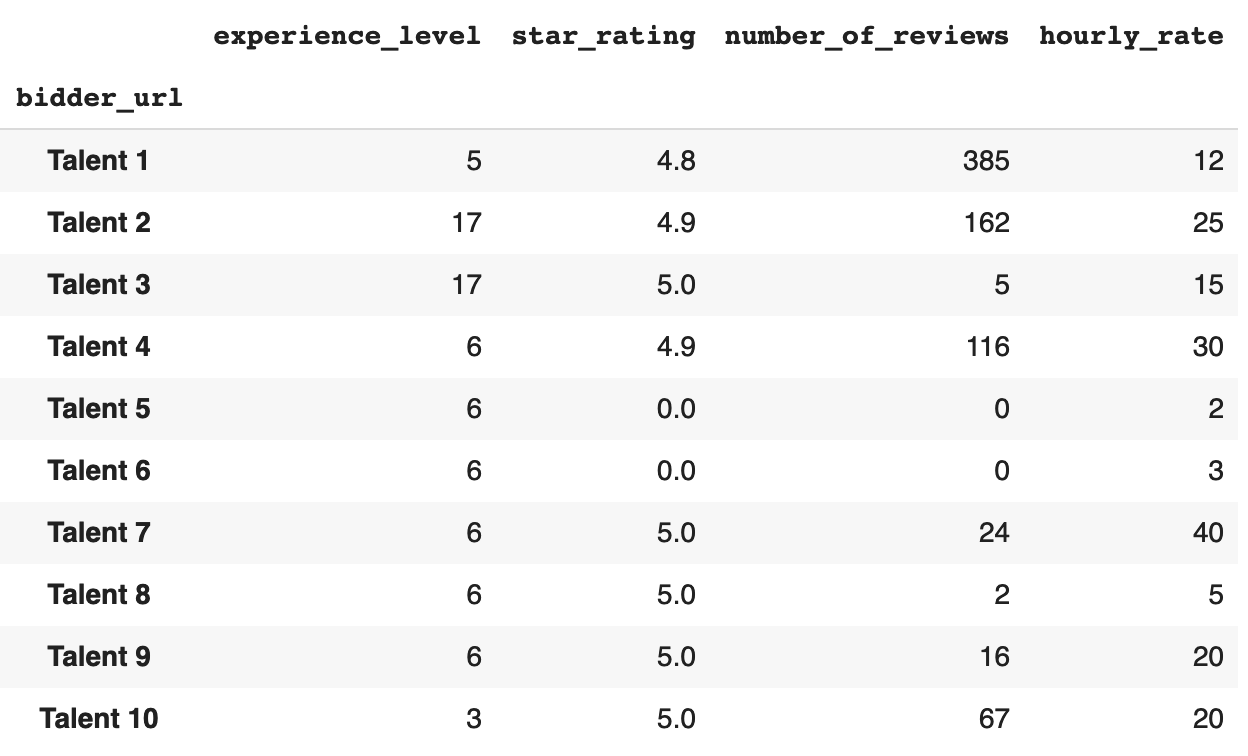
\includegraphics[width=0.75\textwidth]{figures/FreelancerTalentMeta.png}
	\caption{The talent extra information matrix from freelancer.com}
	\label{fig:freelancer-talent-meta}
\end{figure}

As one would expect, the model tries to guess if the person should be employed or not. Out of the \textit{321225} data points in total, we use 60\% for training, 20\% for test and the rest for validation. We split the data into those sets randomly using \textit{train\_test\_split} function of \textit{scikit-learn}. An important parameter not to miss is \textit{stratify}; since our dataset has  6\% positive and 94\% negative samples, we need to make sure that this ratio also remains in the sets. Not using this feature could result in the model always predicting the same negative results. Doing that means that the model would learn the same result, no matter what ~\parencite{singh2015survey}.

After splitting the data, we can start with training. There also exists some important features that we need to use; these optional features all have different objectives, but they all serve to improve the results. These features are all supported by the packages \textit{Keras} and \textit{TensorFlow}, which are open-source neural network libraries. Keras is an abstraction layer for TensorFlow that lets the users train neural networks with a minimal number of lines ~\parencite{chollet2018deep}. While fitting the model with training data, Keras gives the option to add callbacks. The callbacks that we adopt are \textit{EarlyStopping}, \textit{ModelCheckpoint},  \textit{ReduceLROnPlateau} and \textit{TensorBoard} . As the name suggests, early stopping [TODO: add neural networks to research part; also validation loss, overfitting, graph vs] serves to prevent overfitting. In our case, it compares the validation loss of current batch with the previous one. If the validation loss doesn't drop for ten times, the training stops. The next callback model checkpoint is used complementary to early stopping. Model checkpoint saves the model weights of the batch with the minimum validation loss. After the training is complete, we load those model weights that achieved the best accuracy. ReduceLROnPlateau reduces learning rate when the validation loss has stopped improving. Lastly, TensorBoard is a visualization tool for TensorFlow. It produces model visions and graphs that show the evolution of the accuracy, loss and learning rate. 

When we are training the model, we should also set the training weights for both labels manually. The dataset encompasses 6\% positive and 94\% negative samples, so we need to penalize the errors according to this rate. After training, the class weights are ignored and not used in testing/predicting.


The figure \ref{fig:tensor-board-sparse}  depicts the model that is used to predict if a talent should be employed or not. The direction of the graph starts at the bottom of the image and goes up. Like it was mentioned before, the model expects three feature vectors. These vectors are defined as the skill vectors of the project, the skill vector of the talent and extra information of the talent(e.g., hourly rate, total experience). 

 \begin{figure}[!ht]
	\centering
	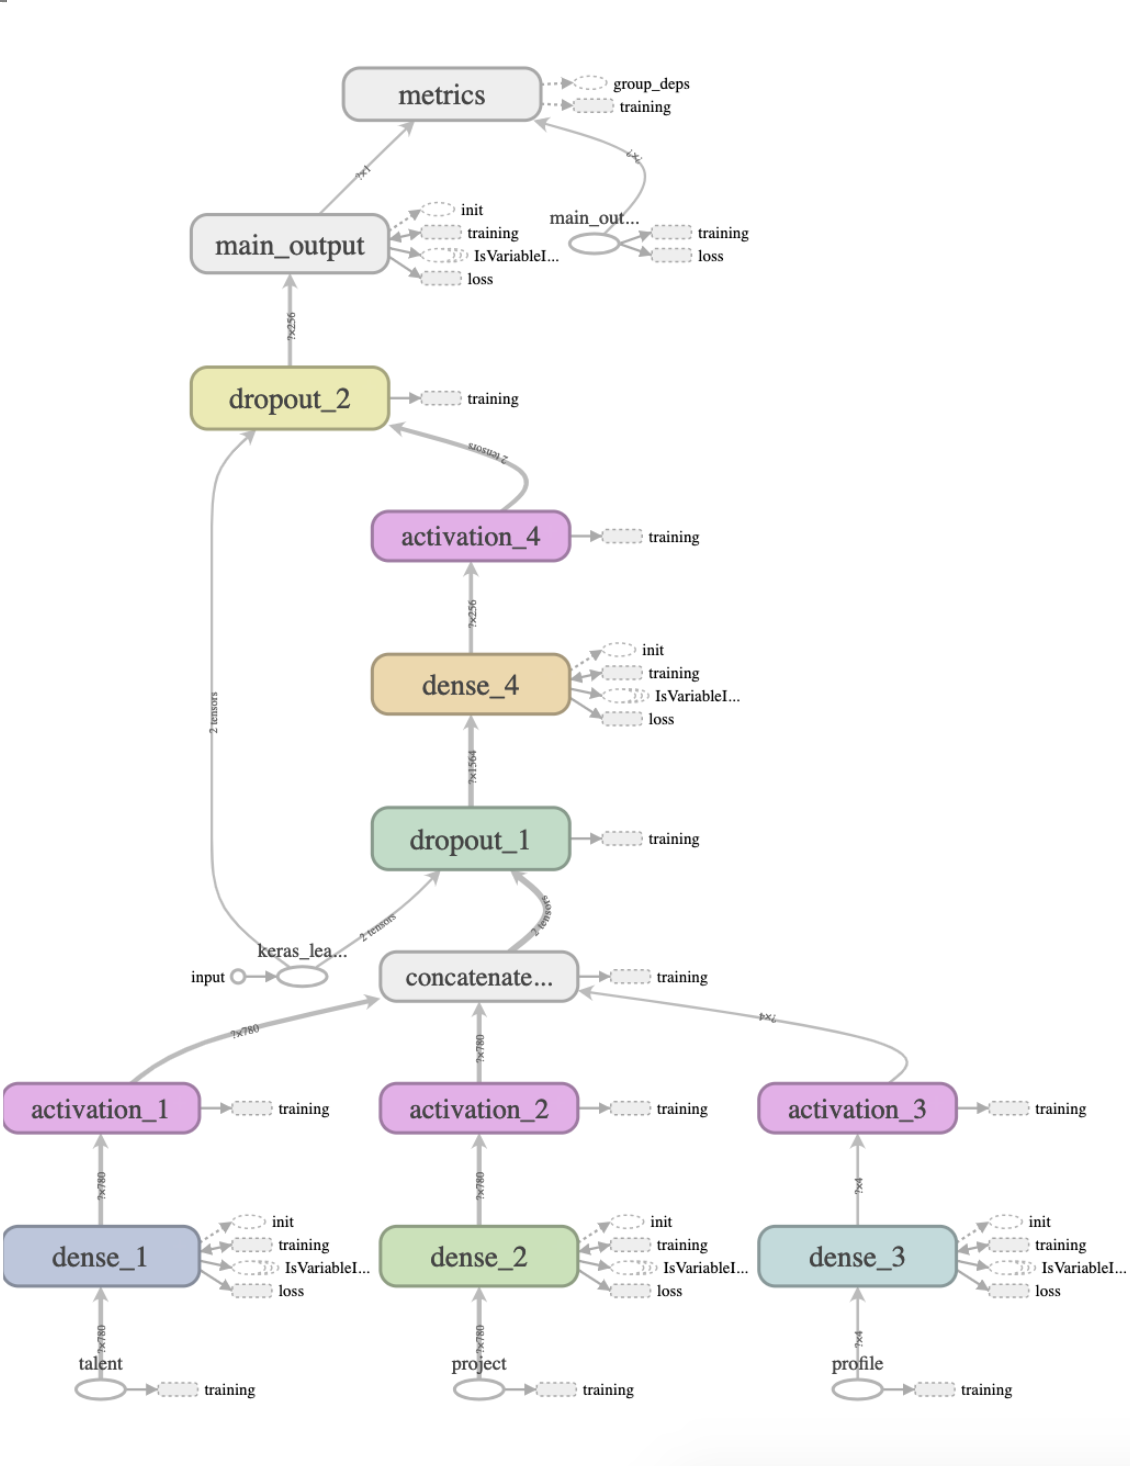
\includegraphics[width=0.75\textwidth]{figures/TensorBoardSparseCropped.png}
	\caption{The graph that explains the sparse input model}
	\label{fig:tensor-board-sparse}
\end{figure}

For each of the inputs, a dense layer exists with the number of neurons equal to the number of features. Making this decision means that project and talent layers contain 780 neurons and profile information layer contains four neurons. For these layers, we use \textit{relu} activation, \textit{l1} regularization with the value \textit{0.0001} and we initialize the weights with \textit{he normal}. Detailed knowledge about activation, regularization, and weight initialization can be found in the ~\autoref{chapter:review_of_research}[TODO: add activation, regularization, and weight init to research chapter].



After the activation functions, all layers get concatenated horizontally. Concatenation layer is followed by a dropout layer with half of the neurons are disabled randomly[TODO: add dropout to neural networks section of chapter 2]. Next one in the model is a dense layer with 256 nodes, which possesses the same activation function, regularization and weight initialization methods as the previous dense layers. The model accommodates the last dropout layer and ends with the main output. The output is only a one node layer and involves a \textit{sigmoid} activation function that squeezes the output value to be between 0 and 1[TODO: research -> nn -> activation functions -> sigmoid]. The weight initializer of the last layer is \textit{glorot uniform}.[TODO: research -> nn -> weight initializers -> glorot uniform].

\begin{equation}
C(w, b) \equiv \frac{1}{2 n} \sum_{x}\|y(x)-a\|^{2}
\label{eq:mean-squared-error}
\end{equation}

Each neural network has the aim of minimizing its cost function ~\parencite{Goodfellow-et-al-2016}. The cost function that we chose is \textit{mean squared error}[See ~\autoref{eq:mean-squared-error}]. This example of the cost function is used mostly for regression tasks and calculates the mean squared difference of the actual value and the predicted output value. The metric we use is accuracy, and more information about it can be found in ~\autoref{chapter:evaluation}.


\subsection{Using Embeddings}\label{subsection:using-embeddings}

High-dimensional spaces and distributions prove to be unexpected and completely differ from low-dimensional spaces. The empty space phenomenon and other ones are examples of the \textit{curse of dimensionality}. With the help of embeddings layers, we can represent high-dimensional data in low-dimensions  ~\parencite{lee2007nonlinear}.


Although deep neural networks can avoid the curse of dimensionality ~\parencite{poggio2017and}, we still need to use embeddings layers for spatial reasons. In the previous sections, we mentioned that there are 780 unique skills for freelancer data and 923 skills if we also add Motius data. Having all of this data means that the data has 923 dimensions and we know that the information is sparse, most of the data matrices consist of zeroes so that we can reduce the dimensionality. 

[TODO explain embeddings in research. also explain embeddings math. instead]
 \begin{figure}[!ht]
	\centering
	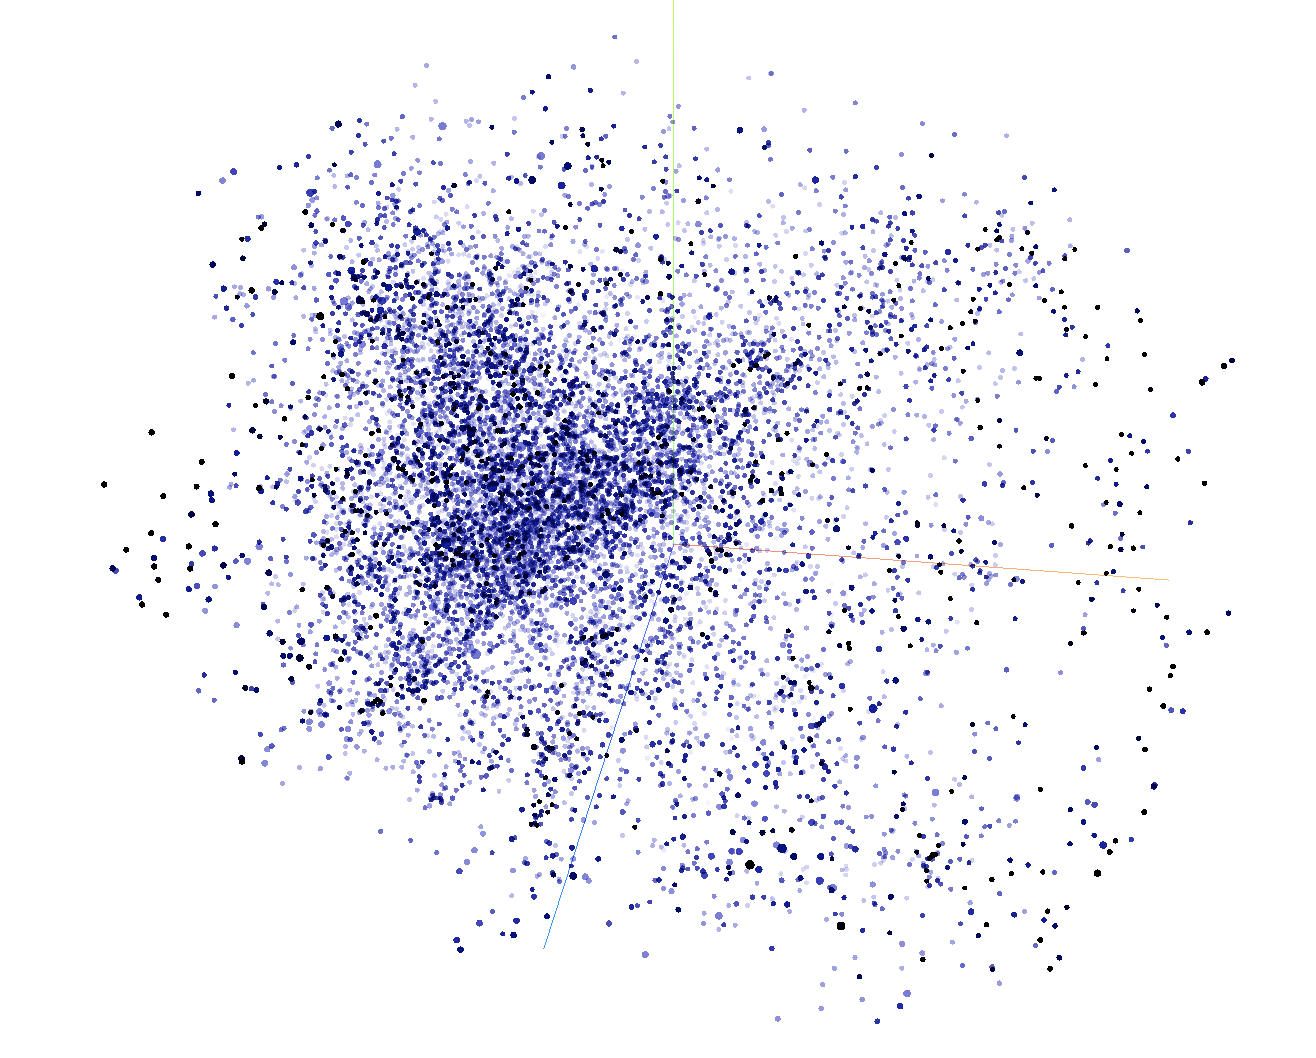
\includegraphics[width=0.75\textwidth]{figures/EmbeddingThesis.png}
	\caption{3D version of the embedding space that is created for projects of this thesis}
	\label{fig:embedding-projection}
\end{figure}


\subsubsection{Preprocessing}

For both Freelancer and Motius data, we know the skill levels of projects and talents for various skills. Instead of having some positive and hundreds of zero skill values for each project/talent, we can set a skill threshold. This threshold implies skills above or equals to the limit are positive, and the rest are zero. The idea is converting the talent-skill and project-skill matrices so that, each talent/skill holds a list of skills they know/require. However, another constraint that needs to be addressed is the maximum length of the padded skill matrix, because neural networks require a fixed input shape. Therefore, the talent/project maximum amount of positive skills is determined. For Freelancer data, this is 18, which means all skills vectors are padded with zeroes to have the length of 18. 

In the case of Motius data, the topic is more complicated. The ~\autoref{subsection:company-dataset} explained how the correlation mechanism of the company data works. To describe it briefly, Motius stores user skills and other skills that are correlated for each user. Including this data affects that there exist many skills for each user, but most of these skill levels are low. Here the highest skill level would 2, and the smallest would be 0.



\begin{figure}[htpb]
	\centering
	
	\pgfplotstableset{col sep=&, row sep=\\}
	% This should probably go into a file in data/
	\pgfplotstableread{
		a & b    \\
		0.1 & 780 \\
		0.2 & 732 \\
		0.3 & 676 \\
		0.4 & 605 \\
		0.5 & 530 \\
		0.6 & 463 \\
		0.7 & 386 \\
		0.75 & 361 \\
		0.8 & 325 \\
		0.9 & 299 \\
		1.0 & 269 \\
	}\exampleA
	\pgfplotstableread{
		a & b    \\
		0.1 & 132 \\
		0.2 & 112 \\
		0.3 & 94 \\
		0.4 & 71 \\
		0.5 & 57 \\
		0.6 & 44 \\
		0.7 & 28 \\
		0.75 & 21 \\
		0.8 & 16 \\
		0.9 & 12 \\
		1.0 & 9 \\
	}\exampleB
	% This should probably go into a file in figures/
	\begin{tikzpicture}
	\begin{axis}[
	ymin=0,
	legend style={legend pos=outer north east},
	grid,
	thick,
	ylabel=Threshold,
	xlabel=Amount
	]
	\addplot table[x=a, y=b]{\exampleA};
	\addlegendentry{Amount of Motius talents};
	\addplot table[x=a, y=b]{\exampleB};
	\addlegendentry{Maximum skill vector length};
	\end{axis}
	\end{tikzpicture}
	\caption[Threshold figure]{Effect of threshold selection on talents and maximum skill vector length}\label{fig:threshold-selection}
\end{figure}

The effect of different threshold values on Motius data is shown on \autoref{fig:threshold-selection}. Without any threshold, there is a couple of Motius projects with the maximum skill length of 21. Projects don't specify skill levels, so these are taken as they are. That's why we also wanted to have a similar maximum length for Motius talents. When there is no threshold, there are 780 Motius talents with at least one skill value, but the maximum skill vector length is 132. We wouldn't want to implement this version because the maximum range of 132 will create millions of zeroes in the dataset, which we tried to avoid in the first place. Setting the threshold to a high value(like 1 or more) is also not optimal since it limits the maximum skill vector length to 9 and number of Motius talents to 269. Having such a high value would decrease the amount of information we have significantly because the Freelancer data also has a maximum length of 18. Therefore, the optimum threshold value we reached is \textit{0.75}. Doing this limits the number of Motius talents to 361 and limits the maximum skill vector length to 21, just like the project with the most skills.

\autoref{fig:embedding-training-matrix} depicts the training data with full skill matrix. The columns with the numbers in range 0 to 20 are the indices of the talent skills and the columns with the names 21 to 41 are project skills indices.  The version of the image is the one with the Motius and Freelancer data combined. In the variant with only Freelancer data, we have skill vector lengths of 18 and the extra information of talents included.

 \begin{figure}[!ht]
	\centering
	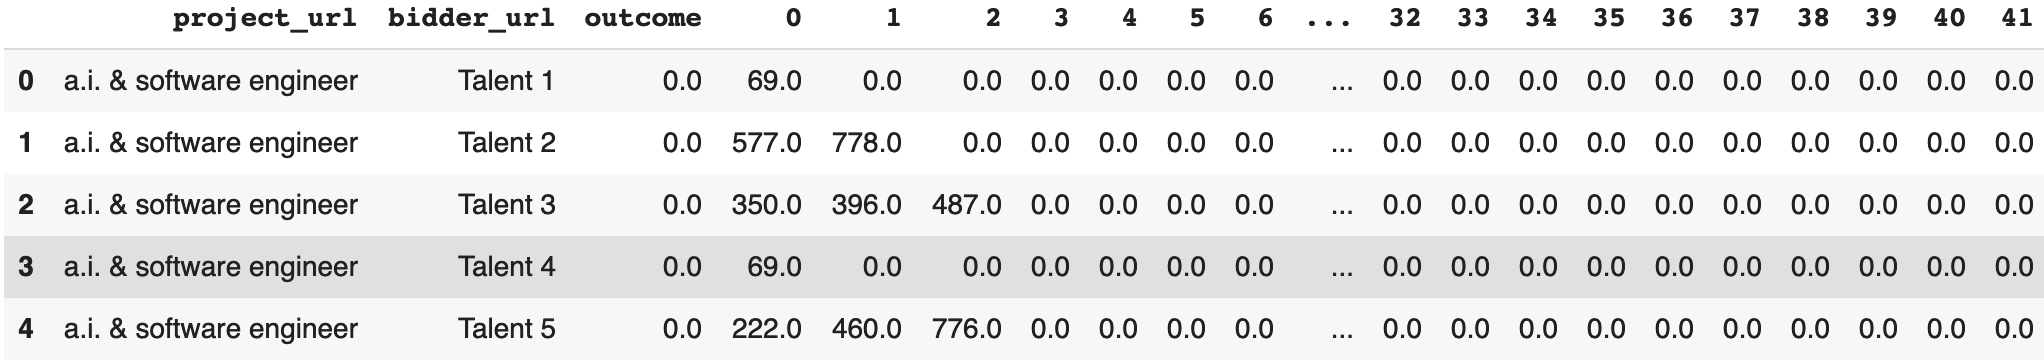
\includegraphics[width=\textwidth]{figures/EmbeddingTrainingMatrix.png}
	\caption{Training data that contains padded embedding skill vectors}
	\label{fig:embedding-training-matrix}
\end{figure}



\subsubsection{Simpler Architecture for Company Dataset}

The Freelancer dataset has a huge advantage over Motius data, which is the extra information that we know about the applicants. When we use both datasets together to train a model, we can limit the inputs to talent and project skills. 

\autoref{fig:model-code} illustrates the simplified version of the \textit{Python} code that constructs the model to predict the hiring result. The \textit{features} parameter of the model building function corresponds to the length of the padded skill vector and the next parameter \textit{dimensions} represents the total amount of unique skills. Embedding layers in Keras expect the arguments \textit{input dimension}, \textit{output dimension}, \textit{input length} and the optional flag \textit{mask zero}. As embeddings only accept positive integers, input dimension should be the size of the vocabulary, which is the number of total skills in the recommender system. The value of the output dimension can be decided by the developer and explains the size of the desired output dimension. Although no scientific document states an ideal output dimension, the trial-and-error method showed that the best result is achieved with the fourth root of the number of dimensions. The additions of one in multiple places in the code are due to using the mask zero operation. Zeros in rows get filtered out, which increases the performance and speeds up the training process. The cost function that we use is \textit{binary crossentropy} because we want to optimize the process of hiring or not hiring talent to the project. [TODO: research -> cost functions -> binary crossentropy]. Lastly, \textit{sigmoid} activation function squeezes the output value to be between 0 and 1[TODO: research -> nn -> activation functions -> sigmoid].


\section{Unsupervised Group Recommender}\label{section:unsupervised-group-rec}

In this section, we explain the process of recommending multiple talents to supergroups. The methods that are used for this part are derivations of the ones that are used in individual recommenders. Therefore, the basic concepts that are employed before also apply here. 

To perform group recommendations, project-role or project-project information are needed. The website freelancer.com shows other projects from the same supervisor, which can be combined. Then these projects will form a super project and projects can be treated as roles of a more significant project. For Motius data, we already possess this information as project-role data. Roles of Motius correspond to the projects in the Freelancer data. In terms of simplicity and shortness, we only take Freelancer dataset with groups of size five into account. 

\subsection{Baseline}

The basic approach to unsupervised group recommendations would be calculating the cosine similarity between each project and talents. Then pick the best talents and listing them. However, the results won't be diverse, and we can pick talents that have similar skills to each other. We want to avoid that [TODO add different evaluations to both theory and their results to the evaluation part!] and have diverse recommendations for each project.


\subsection{Diverse}\label{implementation-diverse}

Because of the reasons above, we want to create the recommendation list in a diverse way from the beginning. The topic of diversity is already explained before[TODO: research -> diversity enhancement] and the pseudocode to enhance diversity is shown below.

\begin{equation}
\begin{array} { l } { R \leftarrow \emptyset } \\ {  while\, | R | < k\,: } \\ { \quad i * \leftarrow \arg \max _ { i \in C - R } g ( R \cup \{ i \} , \lambda ) } \\ { \quad R \leftarrow R \cup \{ i * \} } \\ { end\, while\,  } \\ {  return\,  R } \end{array}
\label{eq:diversity-enhancement}
\end{equation}


In the algorithm above, we first create an empty recommendation list \textit{R} and set a recommendation length \textit{k}. In our example, we only consider the groups with project amount of 5, so \textit{k} is five as well. After that, we find the optimal candidate that hasn't been selected yet, is relevant to the project at hand and is also diverse to the other selected candidates. Finding the optimal candidate can be tuned with the help of \autoref{eq:diversity-equation}. The $\lambda$ parameter in the equation can be optimized to value the relevancy or diversity more; $\lambda$ of 1 means to only consider variety, 0 factors to consider relevancy and 0.5 gives the balanced result. When we receive the optimal candidate from the equation, we add them to the recommendation list and iterate until we have enough talents for the whole group.

\begin{equation}
g ( R , \lambda ) = ( 1 - \lambda ) \frac { 1 } { | R | } \sum _ { i \in R } f _ { r e l } ( i ) + \lambda d i v ( R )
\label{eq:diversity-equation}
\end{equation}

When we compare the diversity of the baseline approach to the diverse group recommendation, it is obvious that the diversity of talents recommended has increased. The evaluation algorithm for diversity and other relevant measures can be found in \autoref{chapter:evaluation}. [TODO group-rec evaluation]

\section{Supervised Group Recommender}\label{section:supervised-group-rec}

The previous section was about performing group recommendations with unsupervised learning. This section will do the same job using a supervised learning model that we used in \autoref{section:supervised}.


\autoref{eq:diversity-equation} includes a $f _ { rel } $, which is a relevancy score and a diversity rate that can be computed via cosine similarity, neural networks or other methods. In contrast to the unsupervised method, we calculate the relevancy score using the neural network that we used in \autoref{section:supervised}.

What we do in the individual supervised learning part is, training all parameters jointly, which is called end-to-end learning. This ideal was also the first aim for supervised group recommender approach. However, the data for such knowledge doesn't exist. To apply it, we would need data of hiring decisions for the groups not just projects. Since we don't have such information, we would have to generate it with a separate algorithm. In the end, it wouldn't bring much, because the model would learn the data generation algorithm and wouldn't have an effect on the real-life hiring prediction.


Due to the reason above, step by step learning process practiced. The first step of the process is training the model to optimize the individual hiring of talents. Then, we predict the relevancy score for each project-talent pair. For diversity score, we use the cosine similarity between the talents. After set those functions, the algorithm \ref{eq:diversity-enhancement} is applied.


In the end, this method increases diversity according to the evaluation methods that are listed in \autoref{chapter:evaluation}.

\section{Group Recommendation using clustering}

Clustering is the process of dividing data into different groups. To perform different multi-project recommendations, we can pick talents from clusters. Therefore, we can be sure that they are dissimilar. 

Since k-means clustering can suffer from the curse of dimensionality~\parencite{steinbach2004challenges} [TODO research: the curse of dim, clustering ve k-means, PCA ekle], To prevent it, it is logical to reduce the dimensionality first. The choice of the author to reduce dimensionality is \textit{Principal Component Analysis}.

The central idea of principal component analysis (PCA) is to reduce the
dimensionality of a data set consisting of a large number of interrelated
variables, while retaining as much as possible of the variation present in
the data set. This idea is achieved by transforming to a new set of variables,
the principal components (PCs), which are uncorrelated, and which are
ordered so that the first few retain most of the variation present in all of
the original variables~\parencite{jolliffe2011principal}. 

 \begin{figure}[!ht]
	\centering
	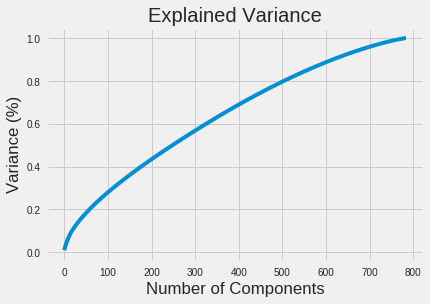
\includegraphics[width=0.75\textwidth]{figures/PCAExplainedVariance.png}
	\caption{Explained variance ratio for difference number of PCs is shown.}
	\label{fig:pca-explained-variance}
\end{figure}

To determine the number of PCs, we can check the explained variance ratio for the different amount of PCs. \autoref{fig:pca-explained-variance} shows how much variance information we lose if we set the number of components to a specific value. Here, it makes sense to note that a higher number will affect the clustering model negatively and a lower number won't be able to capture everything in the dataset. The author of the thesis experimented with different values.

\begin{equation}
a(i)=\frac{1}{\left|C_{i}\right|-1} \sum_{j \in C_{i}, i \neq j} d(i, j)
\label{eq:silhouette-a}
\end{equation}

\begin{equation}
b(i)=\min _{i \neq j} \frac{1}{\left|C_{j}\right|} \sum_{j \in C_{j}} d(i, j)
\label{eq:silhouette-b}
\end{equation}

\begin{equation}
s(i)=\frac{b(i)-a(i)}{\max \{a(i), b(i)\}}
\label{eq:silhouette-c}
\end{equation}

K-means clustering requires a \textit{k} value that determines the number of clusters the model is going to create. The ideal number of clusters can be verified by calculating the silhouette scores for a different number of clusters. The figure \ref{fig:pca-silhouette} shows silhouette scores for different cluster amounts. Silhouette score calculates how similar a data point to its cluster compared to other clusters \parencite{rousseeuw1987silhouettes}. For this task, we use the equation in the equations \ref{eq:silhouette-a}, \ref{eq:silhouette-b}, \ref{eq:silhouette-c}. In the equations, different distance metrics can be employed. The choice of the author is euclidian distance[TODO: distance metrics research].  The equation \ref{eq:silhouette-a} calculates mean intra-cluster distance for each sample and the next \ref{eq:silhouette-b} computes mean nearest-cluster distance for each sample, which means the distance between a sample and the nearest cluster that the sample is not a part of. The last function \ref{eq:silhouette-c} converts the results of the first two equations into silhouette coefficients. The mean of all silhouette coefficients from every sample gives the silhouette score for that \textit{k} value. Higher silhouette scores suggest that the samples well matched to its cluster and poorly matched to neighboring clusters. In the example of \ref{fig:pca-silhouette}, it makes sense to select a value like 30. To visualize results, we project the centers of the clusters  on a 2D space[See \ref{fig:kmeans-centers}]. The X-axis of the graph is the maximum value in each cluster center coordinate, and the Y-axis of the graph is the maximum value in each cluster center coordinate.

 \begin{figure}[!ht]
	\centering
	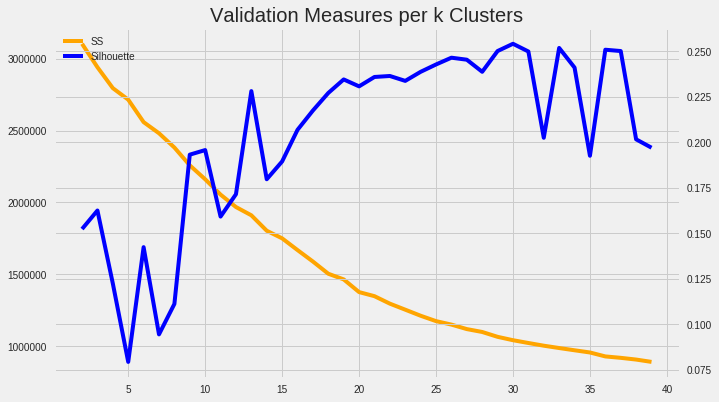
\includegraphics[width=\textwidth]{figures/PCASilhouette.png}
	\caption{Silhouette scores of many different \textit{k} values of k-means}
	\label{fig:pca-silhouette}
\end{figure}


Next, we benefit from another function of the PCA; \textit{inverse\_transform}. Inverse transform takes the cluster centers as an input and converts them to full talent values. This conversion promises that we treat each cluster center like talent and transform their values to skill values and extra information. In end, we possess an average skill vector for every cluster [See figure \ref{fig:cluster-centers-matrix}]. The figure contains some part of the skill vectors of the first three average talents. For example the cluster(segment) 0 in the figure has exceptional \textit{Adobe Illustrator} skills. Segment 1, on the other hand, is an all-rounder. Lastly, segment 3 is a \textit{c\#} developer.  It must be noted these values are calculated after standard scaling[TODO research -> standard scaling].

 \begin{figure}[!ht]
	\centering
	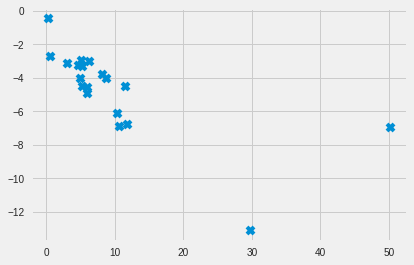
\includegraphics[width=0.75\textwidth]{figures/KMeansCenters.png}
	\caption{Centers of clusters that are projected on a 2D space}
	\label{fig:kmeans-centers}
\end{figure}


After we exercise clustering, we can start with the group recommendation process. The recommendation can be operated both supervised[See \ref{section:supervised-group-rec}] or unsupervised[See figure \ref{section:unsupervised-group-rec}]. The same principles apply, and we calculate the relevancy score with cosine similarity or neural networks. In contrast to the other methods, the algorithm computes the relevancy score of the project and average cluster skills [See figure \ref{fig:cluster-centers-matrix}]. This way, we determine the ideal cluster for the project. When a project got recommended a talent from a specific cluster, that cluster is excluded from the next projects in the group. Therefore, diversity in a group is guaranteed. After the selection of the optimal cluster, the best candidate in that cluster is chosen via neural networks or cosine similarity.

 \begin{figure}[!ht]
	\centering
	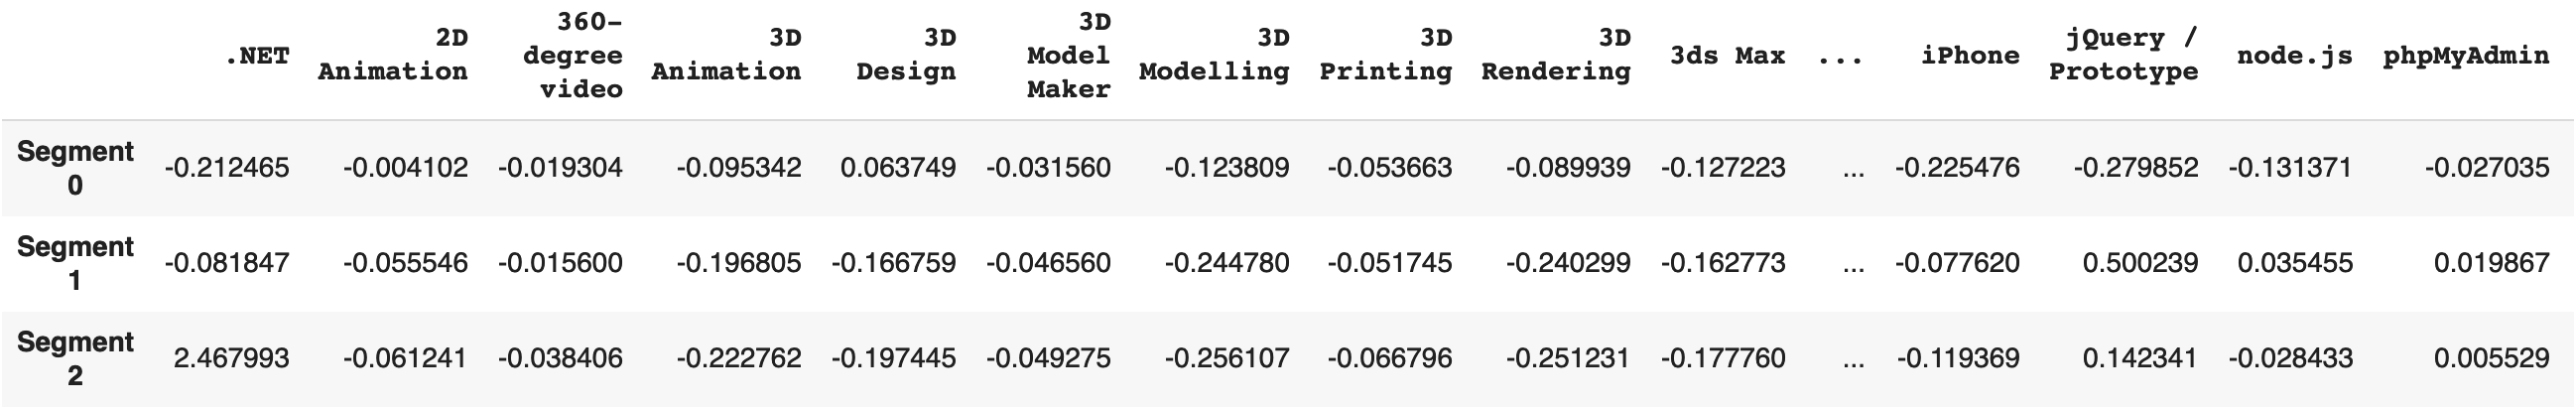
\includegraphics[width=\textwidth]{figures/ClusterCentersMatrix.png}
	\caption{Examples of some centers of clusters that are projected on a 2D space}
	\label{fig:cluster-centers-matrix}
\end{figure}



\section{Dashboard to show data and enter Feedback}

\subsection{General Dashboard}

Another big part of the thesis is the dashboard that was built for various purposes; these purposes are showing individual unsupervised, supervised and hybrid recommendations for Motius and Freelancer datasets, showing group recommendations using unsupervised, supervised and hybrid methods and allowing to enter feedback, that has direct and indirect effects on the results.

The dashboard adopts the front-end that is programmed with \textit{Vue.js} and a back-end that employs \textit{Flask}[TODO: research -> frontend, backend, docker]. Vue.js is a front-end development framework that can be programmed with JavaScript. Flask is a back-end development framework that can be called with Python. The reason to use Vue.js is because of subjective reasons; it a reactive, modern framework that is easy to develop \cite{you2018vue}. Flask is, on the other hand, is chosen, because it is a popular light-weight Python framework \cite{grinberg2018flask}. Since the rest of the machine learning training/prediction was done on Python, the author seized the opportunity to reuse/adapt the same codebase. 

Docker is a container virtualization technology, which like a very lightweight virtual machine. Adding Docker to our software stack gives the advantage of portability. This is important for various reasons; first of all the operating system choice of the author is \textit{MacOS} but most of the servers run different flavors of \textit{Linux}. All of the different operating systems have different installation methods, different pre-installed libraries, and different dependencies. Docker solves this problem by standardizing the building and running operations of virtual machines. This way, the author was able to run everything on own computer and can be sure that it will also run perfectly on the servers of Motius if they choose to implement the solution on their internal system. \cite{anderson2015docker}.


 \begin{figure}[!ht]
	\centering
	
\includegraphics[width=0.5\textwidth]{figures/DashboardMain.png}
	\caption{Main screen of the dashboard}
	\label{fig:dashboard-main}
\end{figure}


The main screen of the dashboard is shown in figure \ref{fig:dashboard-main} and it contains a search box and a dropdown. When users type anything on the search box, the front-end sends a \textit{get request}[TODO: research -> get, post requests]. As the back-end receives the request, it checks the database for the text that is given by the user. Then, the back-end returns relevant projects as a list. 


The dropdown on that screen has three options; \textit{All},  \textit{Motius} and  \textit{Group}. The \textit{all} mode searches the input text in all projects database that includes Freelancer and Motius projects. As the name suggests, Motius mode only returns the company projects, and the group mode returns group numbers, which are a combination of various projects[See figure \ref{fig:dashboard-projects}]. 

 \begin{figure}[!ht]
	\centering
	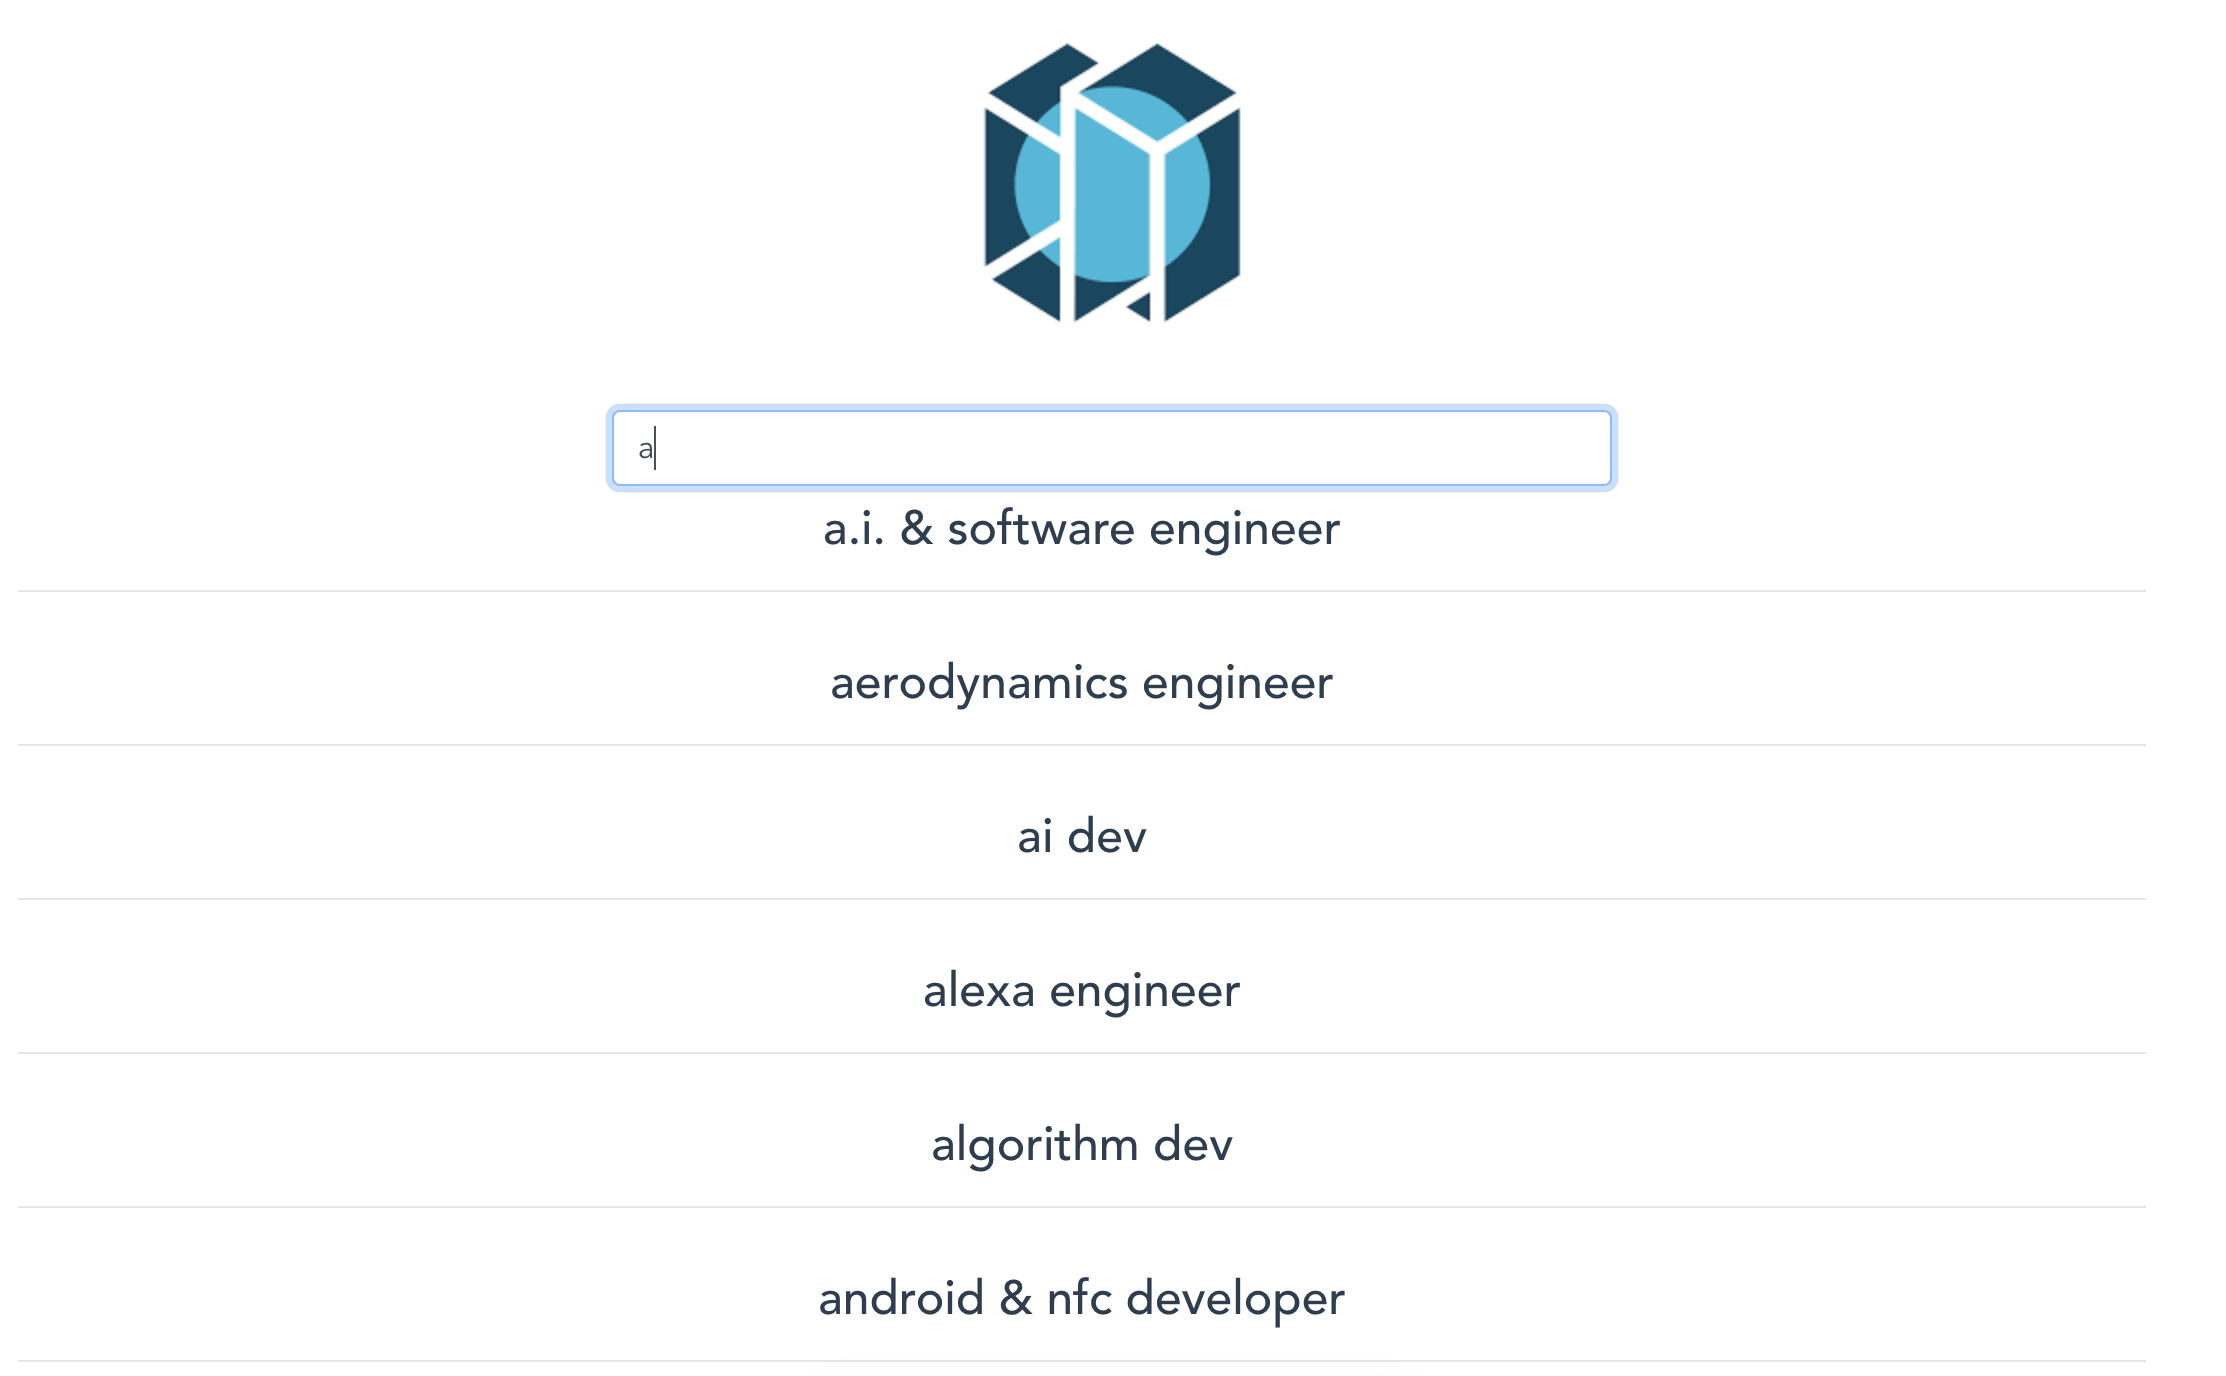
\includegraphics[width=0.75\textwidth]{figures/DashboardProjects.png}
	\caption{A snippet from the list of all projects that start with the letter \textit{a}}
	\label{fig:dashboard-projects}
\end{figure}

\subsection{Individual Recommendations}

When users click on any of the projects that are listed in figure \ref{fig:dashboard-projects}, they receive recommendations with respective scores. For the case of individual recommenders, these scores can be from the neural network model, cosine similarity or hybrid.

The back-end of these different recommenders is all explained in the previous subsections. The figure \ref{fig:dashboard-individual} shows individual recommendations for an artificial intelligence project. There is a dropdown that has choices such as \textit{neural networks}. \textit{cosine similarity} and \textit{hybrid}. Baseline neural networks give individual recommendations that come from the machine learning model. Cosine similarity method checks the angle between talent and project vectors. Lastly, hybrid mode combines neural networks and unsupervised similarity to come up with new predictions.

 \begin{figure}[!ht]
	\centering
	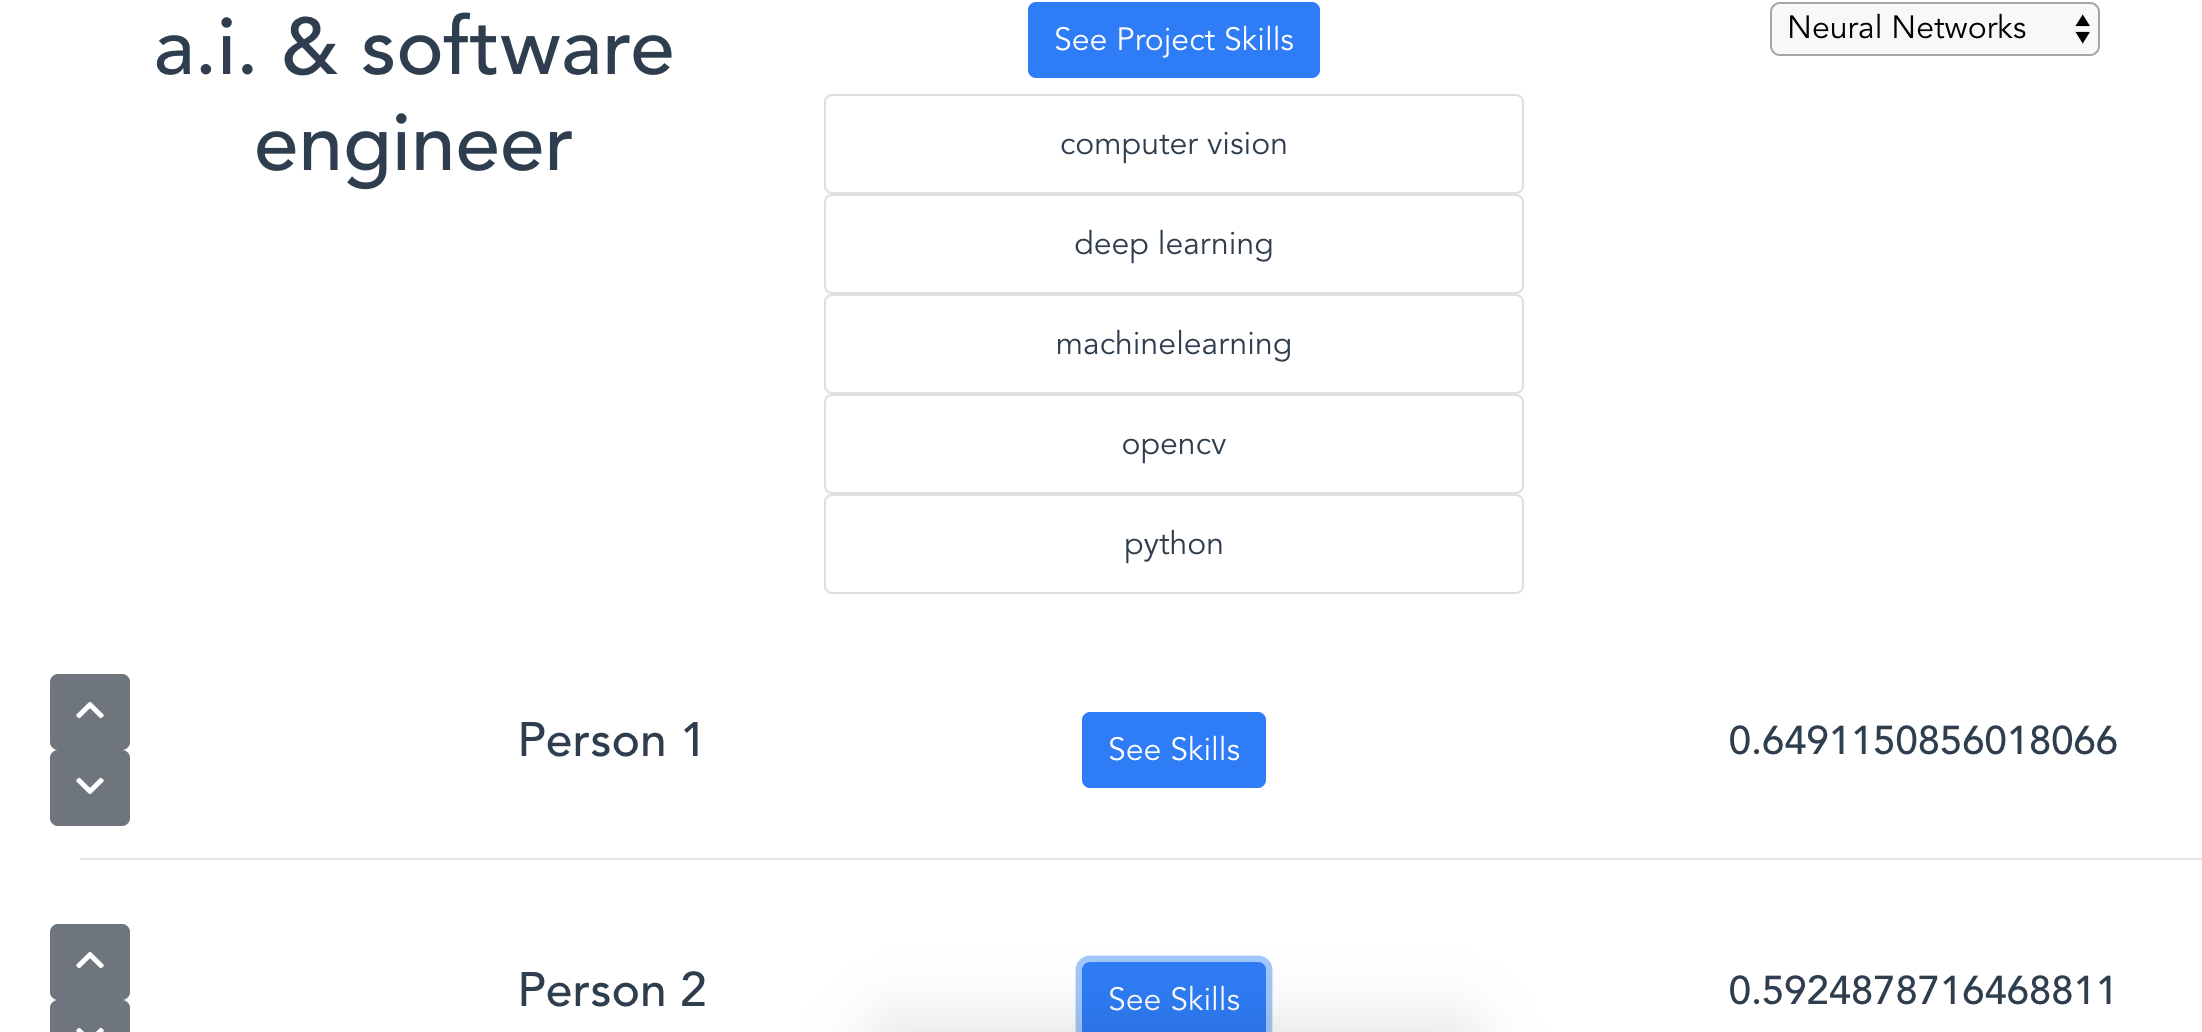
\includegraphics[width=\textwidth]{figures/DashboardIndividual.png}
	\caption{A screenshot from the list of all recommendations from neural networks for the project \textit{a.i. \& software engineer}}
	\label{fig:dashboard-individual}
\end{figure}

\autoref{fig:dashboard-individual} shows the results for the project \textit{a.i. \& software engineer} on the dashboard that is built by the author. Names of the people that were recommended are anonymized, but the rest of the data are real-life. The example project at hand requires the skills \textit{computer vision}, \textit{deep learning}, \textit{machinelearning}, \textit{opencv} and \textit{python}. Although the skills of the person one is not shown(because that person retains 21 skills, which are too long for the figure), person 1 is not the talent with the most overlapping skills. Instead, person 1 is a talent that was recommended the most by the Motius internal recommender. Next, person 2 knows no skills that the project requires. This lack of knowledge aligns with the fact that it is hard to conclude the neural networks and they are mostly referred to as \textit{black-boxes} \cite{benitez1997artificial} [ref TODO evaluation].

 \begin{figure}[!ht]
	\centering
	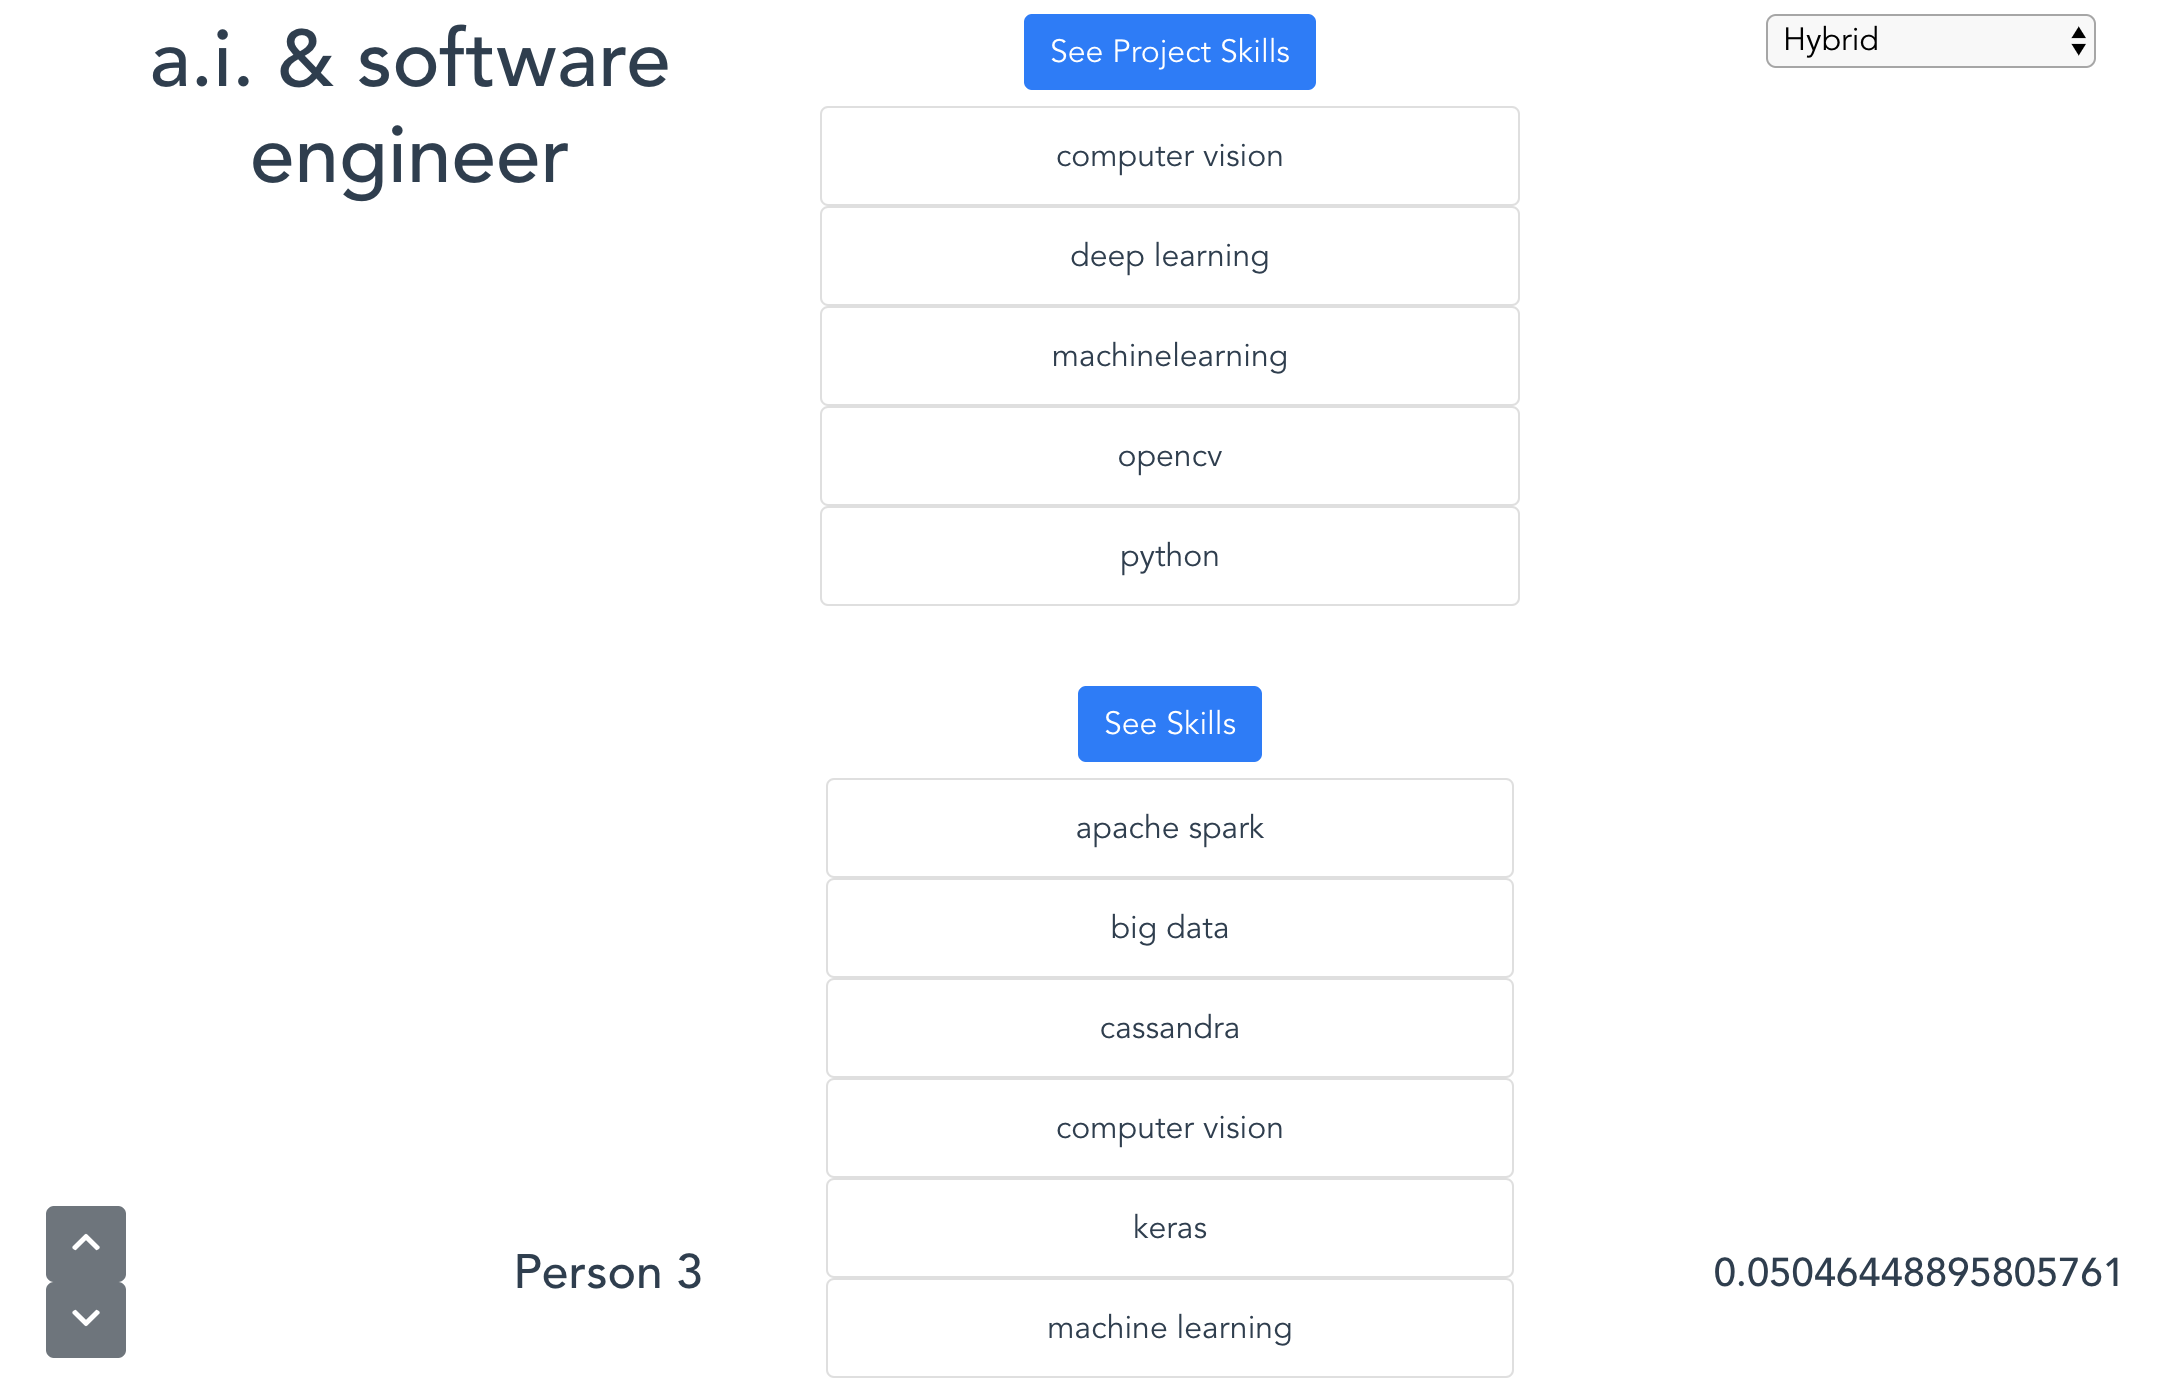
\includegraphics[width=\textwidth]{figures/DashboardIndividualHybrid.png}
	\caption{A screenshot from the list of all recommendations from neural networks for the project \textit{a.i. \& software engineer}}
	\label{fig:dashboard-individual-hybrid}
\end{figure}

In contrast to the figure \ref{fig:dashboard-individual}, figure \ref{fig:dashboard-individual-hybrid} demonstrates the adequate talents for the same project as before. However, people that are listed are different. As it was explained in \ref{section:hybrid}, hybrid practice multiplies the results of from the neural networks and skill vector similarity. This way, the results that are recorded, always have some common skills. In the example, these skills are \textit{computer vision} and \textit{machine learning}.

\subsection{Group Recommendations}

The dashboard also can perform group recommendations. For the case of group recommenders, the scores can be from baseline neural networks, baseline cosine similarity, diverse neural networks or diverse cosine similarity. [TODO: in evaluation-> show screenshots of diverse nn, nn, constant 0 and constant 1 for comparison.]

Baseline cosine similarity, reveal the list of best talents for each project using skill vector similarity and baseline neural networks do the same with neural networks. Diverse cosine similarity and diverse neural networks operate, but they include the likeness of talents for each project to other talents in other projects in the same group.


\autoref{fig:dashboard-group} shows the recommendation results for a real-life group with anonymized names. On the top-right part of the figure, a dropdown can be seen. This dropdown reads \textit{Diverse Similarity}. Other options in the dropdown are \textit{neural networks}, \textit{similarity} and \textit{diverse neural networks}. Meaning of these options is already explained in this section. This selection option makes sure that the chosen talents for each project have similar skills and diverse to each other. Between the group name and recommendation mode, a slider is located. This slider determines the constant for the diversity enhancement formula [See \ref{eq:diversity-equation}]. This diversity constant can be tuned to value the relevancy or diversity more; a value of 1 means to only consider diversity, 0 means to only consider relevancy and 0.5 gives the balanced result. There are also options to check project and talent skills. Last but not least, the dashboard provides the option to rate all talents positively or negatively. This part of the thesis is explained in the next section [See section \ref{section:feedback-learning}].

 \begin{figure}[!ht]
	\centering
	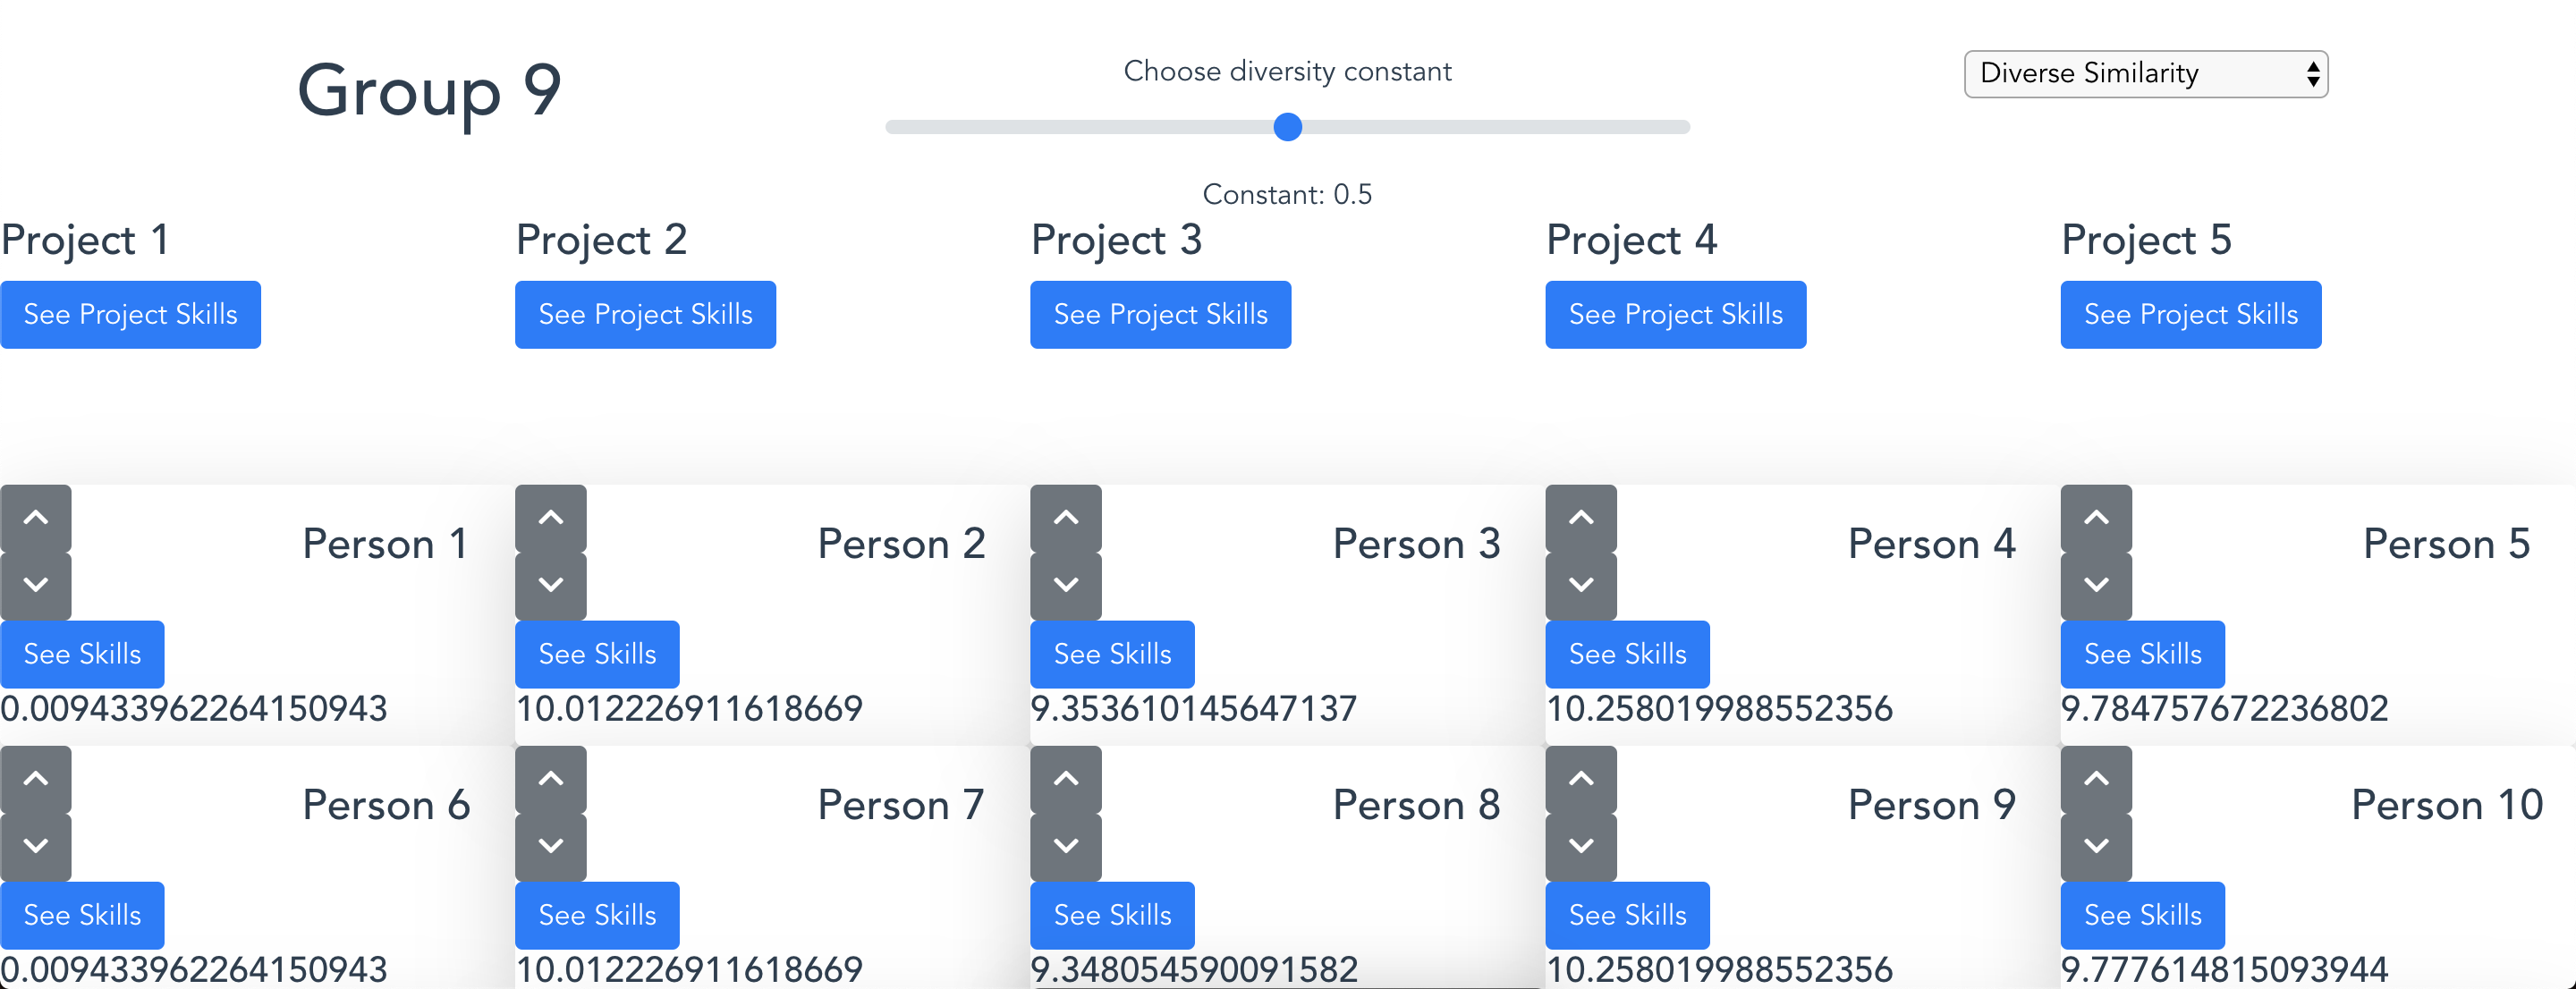
\includegraphics[width=\textwidth]{figures/DashboardGroup.png}
	\caption{A screenshot from the list of all recommendations from diverse cosine similarity for the group 9}
	\label{fig:dashboard-group}
\end{figure}




\section{Improvement of Recommendations via Feedback Learning}\label{section:feedback-learning}

Readers of this thesis may wonder what do the up and down arrows on the figures \ref{fig:dashboard-group}, \ref{fig:dashboard-individual-hybrid} and \ref{fig:dashboard-individual} mean; these arrows correspond to the feedback learning. Recruiters or Human Resources employees that use the dashboard may send positive or negative feedback to every recommendation. 

The feedback that are provided by real people may have direct or indirect effects. To understand the process, it may make sense to check the figure \ref{fig:tensorboard-feedback} first. Feedback data is given to the model as a separate input, and this input is followed by a dense layer with one node with \textit{tanh} activation function. Tanh activation is chosen, because the bias can be negative or positive. [TODO research: tanh]. The output of the bias activation functions is \textit{added} to the result that comes from project-talent information. In this context, adding means actually the mathematical addition operation [See \ref{fig:feedback-model-code}]. Due to this addition, the outcome from the human feedback has a direct effect, even without retraining. 

The default value for any talent bias is 0, and they may be increased up to 1 with positive feedbacks and decrease to -1 with negative feedbacks. These values are added to the result that comes from the dense layer, which gets data from talent and project skills. Since human feedback is stored in the database immediately, they can directly be used and have a direct effect on the total results.


Feedback learning also has an indirect effect;  entering feedback changes the labels of previous training data. This change signifies that positive feedback changes the label of a result to 1(positive) and negative feedback changes it to a 0(negative). That's why, when the developer retrains the model with the new data, it also modifies how the model learns and may also have an impact on other projects.


 \begin{figure}[!ht]
	\centering
	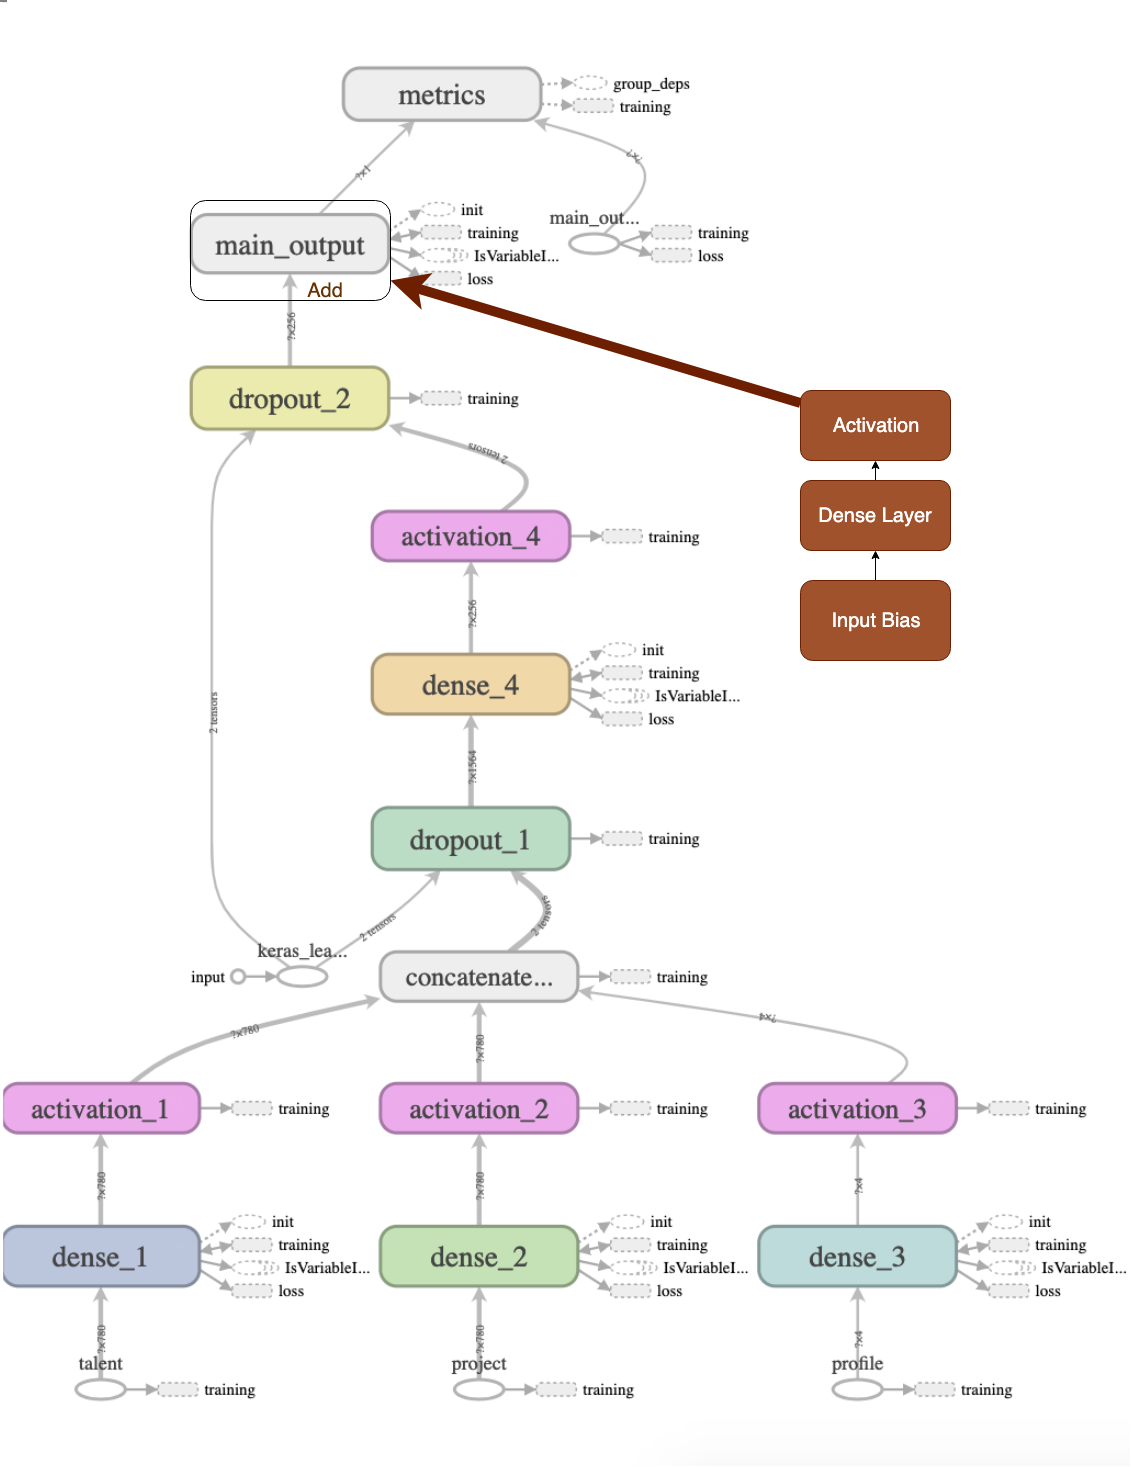
\includegraphics[width=0.8\textwidth]{figures/TensorBoardFeedback.png}
	\caption{Neural networks model with the addition of feedback loop bias}
	\label{fig:tensorboard-feedback}
\end{figure}



\section{Summary}

This chapter analyzed the practical portion of this thesis exhaustively. We explained how we programmed different recommenders with diverse approaches. We also revealed the dashboard that glues everything together and the proposal to improve recommendations with the help of feedback learning. 

The next chapter focuses on the evaluation of the results that were programmed in the scope of this section.

